% filepath: c:\Users\wojte\Desktop\mgr.tex
\documentclass[12pt]{extarticle}
\usepackage[utf8]{inputenc}
\usepackage{geometry}
\usepackage{amsmath}
\usepackage{hyperref}
\usepackage{graphicx}
\usepackage{parskip}
\usepackage{setspace}
\usepackage{float}
\usepackage{amsmath}
\usepackage{enumitem}
\usepackage{amsmath}
\usepackage{amssymb}
\usepackage{geometry}
\usepackage{caption}
\usepackage[utf8]{inputenc}
\usepackage[T1]{fontenc}
\usepackage{amsmath}
\usepackage{amsfonts}
\usepackage{amssymb}
\usepackage{graphicx}
\usepackage[left=2.5cm,right=2.5cm,top=2.5cm,bottom=2.5cm]{geometry}
\title{Neutrino Detection and Data Processing with CNNs}
\author{Wojciech Noskowiak\\}
\date{}

\begin{document}

% --- Thesis Title Page ---
\newgeometry{left=2.5cm,right=2.5cm, top=3cm, bottom=4cm}
\begin{titlepage}
    \centering
    {\Large University of Warsaw \par}
    {\large Faculty of physics \par}
    \vspace{2cm}
    {\large Wojciech Noskowiak \par}
    {\large Record book number: 417909 \par}
    \vspace{2cm}
    {\Huge \textbf{<Title of the diploma thesis>} \par}
    \vspace{2cm}
    {\medium Master's thesis \par}
    {\medium in the field of physics \par}
    \vspace{2cm}
    \begin{flushright} % Shift this block to the right
        {\medium The thesis was written under the supervision of \par}
        {\medium <title/degree, first name and surname> \par}
        {\medium <name of the unit employing the thesis supervisor> \par}
    \end{flushright}
    \vfill
    {\large Warsaw, July 2025 \par}
\end{titlepage}
\restoregeometry

\newpage

% --- Summary Section ---
\section*{Summary}
<Short (maximum 3,000 characters including spaces, but no less than 1,000 characters including spaces) summary of the thesis>

% --- Keywords Section ---
\section*{Keywords}
<List of maximum 10 freely selected words>

% --- Polish Title Section ---
\section*{Title of the thesis in Polish language}
<Title of the thesis translated into Polish language>

\newpage


% \onehalfspacing
% \maketitle
\tableofcontents % Add table of contents
\newpage % Start content on a new page

\section{Introduction}

Neutrino oscillations were first observed in solar and atmospheric neutrinos in the late 1960s and have since been the subject of extensive experimental and theoretical investigation. The mechanism by which neutrinos acquire mass remains insufficiently explained, and the exact values of their masses are still unknown.

In addition, several experimental anomalies have been reported that deviate from the predictions of the three-flavor neutrino oscillation model. These include results from the LSND and MiniBooNE experiments, as well as the reactor neutrino anomaly. In all cases, the observed number of neutrinos does not align with the expectations derived from standard oscillation models.

One possible explanation for these discrepancies involves extending the current model by introducing additional neutrino flavors. In particular, the hypothesis of sterile neutrinos—neutrinos that do not interact via the weak nuclear force—has been proposed. If such a hypothesis would be confirmed it would require an extension of the Standard Model of particle physics. These potential non-interactive neutrinos have even been considered as potential candidates for dark matter.

These anomalies have driven the development of new neutrino detectors designed to probe oscillation phenomena with greater precision. Among them are the MicroBooNE and DUNE experiments.

Efficient analysis and interpretation of data produced by the aforementioned detectors is still an open problem.

This work explores the application of machine learning methods to this problem. Specifically, it investigates and implements selected approaches and evaluates their performance using the publicly available MicroBooNE OpenSamples dataset.

\section{Neutrinos}

Neutrinos are electrically neutral, spin-$\frac{1}{2}$ elementary particles that belong to the lepton family within the Standard Model of particle physics. They exist in three distinct flavors, corresponding to the three charged leptons: the electron neutrino ($\nu_e$), the muon neutrino ($\nu_\mu$), and the tau neutrino ($\nu_\tau$).

These flavor classifications arise from the weak decay processes mediated by the $W$ boson, in which a charged lepton is produced alongside a corresponding neutrino. For instance, in a $W^-$ decay producing an electron, an electron neutrino is emitted; similarly, decays yielding a muon or tau lepton produce a muon or tau neutrino, respectively.

Due to their lack of electric charge, negligible mass, and absence of color charge, neutrinos interact with matter only via the weak nuclear force. This interaction occurs through two fundamental mechanisms: neutral current interactions, mediated by the electrically neutral $Z^0$ boson, and charged current interactions, mediated by the charged $W^+$ or $W^-$ bosons.

In charged current interactions, the neutrino exchanges a $W$ boson with a target particle, resulting in the production of a charged lepton of the same flavor. In contrast, neutral current interactions involve the exchange of a $Z^0$ boson and do not alter the identity of the interacting neutrino.

The weak interaction is characterized by a very short range, typically on the order of $10^{-17}$ to $10^{-18}$ meters, which makes neutrino interactions with matter extremely rare. As a result, detecting neutrinos requires either very intense neutrino beams and/or very large detectors to observe a statistically significant number of interactions.


\section{Neutrino Detectors}

\subsection{Liquid Argon Detectors}

\begin{figure}[H]
    \centering
    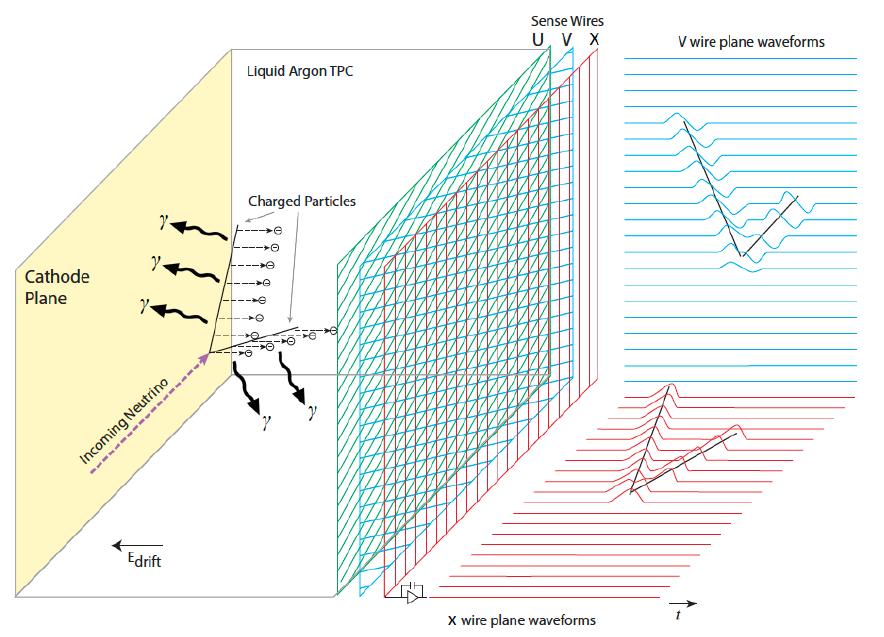
\includegraphics[width=0.7\textwidth]{src/LAr_diagram_DUNE.png}
    \caption{General mechanism of a liquid argon detector (LArTPC).}
\end{figure}

Argon is chosen as the detection medium because it is a noble gas, which is chemically inert and allows for efficient ionization and scintillation. Using argon in a liquid state increases its density, thereby enhancing the probability of neutrino interactions.

LArTPC detectors consist of a large chamber filled with liquid argon. Charged particles traversing the chamber leave trails of ionized electrons. An applied electric field causes these electrons to drift toward the anode, where they are detected. Simultaneously, vacuum ultraviolet (VUV) scintillation photons are emitted and collected by photodetectors.

When a neutrino interacts with an argon nucleus, it produces charged particles that traverse the medium, leaving behind trails of ionized electrons. The detector volume is subjected to a uniform electric field, which causes these free electrons to drift toward a set of anode planes, where their arrival is recorded. At the same time, the interaction generates VUV scintillation photons, which are detected by an array of photodetectors placed around the chamber. The information from the ionization charge provides two spatial coordinates, while the timing information from the scintillation light gives the third coordinate, enabling full three-dimensional reconstruction of particle trajectories and interaction vertices within the detector volume.

\subsection{Noise}

Neutrino interactions are not the only source of signals in the detector. Cosmic rays—high-energy particles from beyond the solar system—can also ionize the detector medium, producing characteristic noise patterns. These patterns are typically distinct and easily distinguishable from genuine neutrino events. They often take the form of long, low-intensity tracks oriented in a single direction. To minimize the occurrence of such noise, LArTPC detectors are usually placed underground. However, complete elimination of these events is not possible.


\section{MicroBooNE Detector}


\begin{figure}[H]
    \centering
    \begin{minipage}[t]{0.48\textwidth}
        \centering
        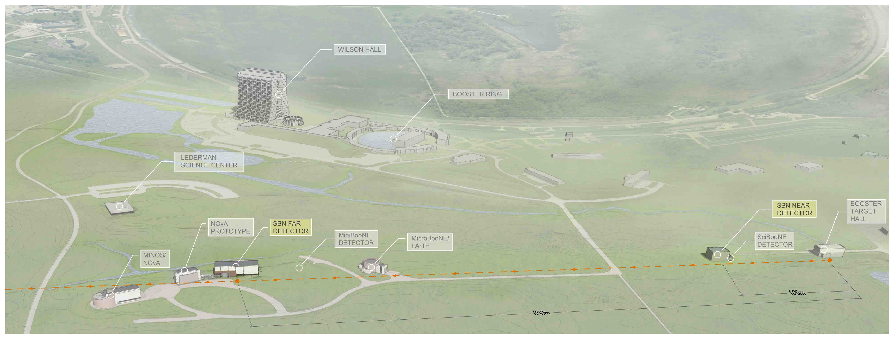
\includegraphics[width=\textwidth]{src/microbooneBirdseyes.pdf}
        \caption{Aerial diagram showing location of MicroBooNE.}
        \label{fig:microboone_birdseye}
    \end{minipage}
    \hfill
    \begin{minipage}[t]{0.48\textwidth}
        \centering
        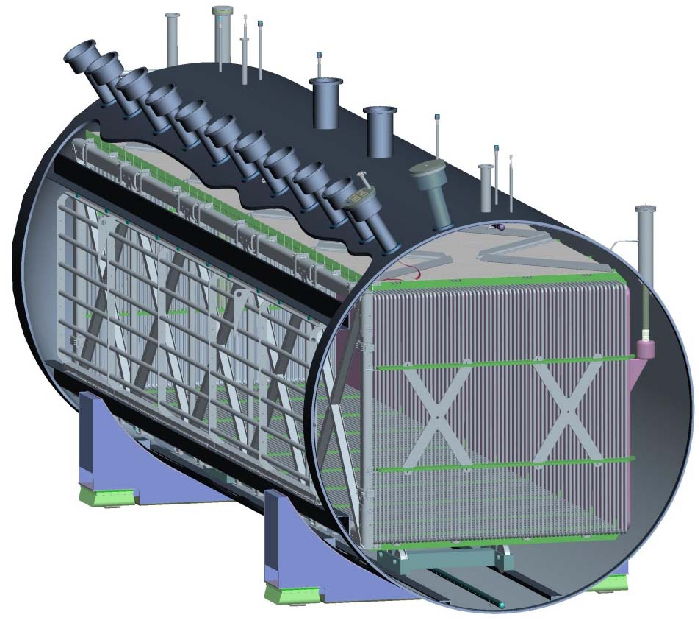
\includegraphics[width=\textwidth]{src/microBooNe_Layout.pdf}
        \caption{Schematic diagram of the MicroBooNE LArTPC inside the cryostat.}
        \label{fig:microboone_layout}
    \end{minipage}
\end{figure}


The MicroBooNE experiment operated at Fermilab from 2015 to 2021 and served as the first detector in the Short-Baseline Neutrino (SBN) program. 

\begin{table}[H]
\centering
\caption{Primary detector design parameters for MicroBooNE.}
\begin{tabular}{|l|l|}
\hline
\textbf{Parameter} & \textbf{Value} \\
\hline
LArTPC Dimensions & 2.325 m vertically \\
                  & 2.560 m horizontally \\
                  & 10.368 m longitudinally \\
\hline
LArTPC argon mass & 90 tonnes \\
\hline
Total Number of Wires & 8256 \\
\hline
Drift field & 500 V/cm \\
\hline
Light collection & 32 200 mm (8 in) diameter PMTs \\
                 & 4 lightguide paddles \\
\hline
Total liquid argon mass & 170 tonnes \\
\hline
Operating temperature & 87 K \\
\hline
\end{tabular}
\label{tab:microboone_specs}
\end{table}

MicroBooNE is based on a 170-ton liquid-argon TPC, enclosed in a cryostat and depicted in Figure~\ref{fig:microboone_layout}. The detector is located on the Fermilab site, as shown in Figure~\ref{fig:microboone_birdseye}. Key design parameters are summarized in Table~\ref{fig:microboone_layout}.

The LArTPC itself contains 90 tonnes of liquid argon. Ionization electrons produced by charged particles traveling through the detector volume are drifted under a uniform electric field of 500~V/cm towards a wire plane assembly. The readout system comprises 8256 wires.

The TPC volume has dimensions of 2.325~m vertically, 2.560~m horizontally, and 10.368~m longitudinally. For light collection, the system includes 32 photomultiplier tubes (PMTs) of 200~mm (8~inch) diameter and 4 lightguide paddles. The detector operates at a cryogenic temperature of 87~K.

In addition to its primary scientific goals, it contributed essential input toward the development of kiloton-scale liquid-argon time projection chambers (LArTPCs) for the upcoming Deep Underground Neutrino Experiment (DUNE).

% 1. Rozdział 3: Change title and add intro about datasets used
\section{MicroBooNE Public Datasets}
At the core of this work are two publicly available datasets from the MicroBooNE experiment: the \textbf{Inclusive} sample and the \textbf{Electron Neutrino} sample. The Inclusive sample contains both charged-current (CC) and neutral-current (NC) interactions, as well as various neutrino types, reflecting the true composition of the Booster Neutrino Beam. The Electron Neutrino sample, on the other hand, contains only electron neutrino CC interactions.

% 2. Section 2.5: Add one sentence about each file format and cite sources
The MicroBooNE OpenSamples dataset is provided in two formats: HDF5 and art/ROOT. The \textbf{HDF5} format is a hierarchical data format suitable for efficient storage and access to large numerical datasets. The \textbf{art/ROOT} format is based on the ROOT framework, which is commonly used in high-energy physics for storing and analyzing complex event data structures~\cite{hdf5,root}. 

% 3. Section 2.5: Add sentence about "wires" vs "no wires"
There are two main types of data samples: \textbf{with wires} and \textbf{no wires}. The "with wires" datasets include full waveform data from the detector wires, allowing for signal reconstruction and image generation. The "no wires" datasets omit this raw waveform information, providing only data collected from scintillators.


\subsection{Events Present in the Dataset}

The distributions of lepton and neutrino energies for the two datasets are shown in Figures~\ref{fig:lepton-inclusive}--\ref{fig:neutrino-nue}. Each figure caption specifies which dataset is being visualized.

\begin{figure}[H]
    \centering
    \begin{minipage}[t]{0.6\textwidth}
        \centering
        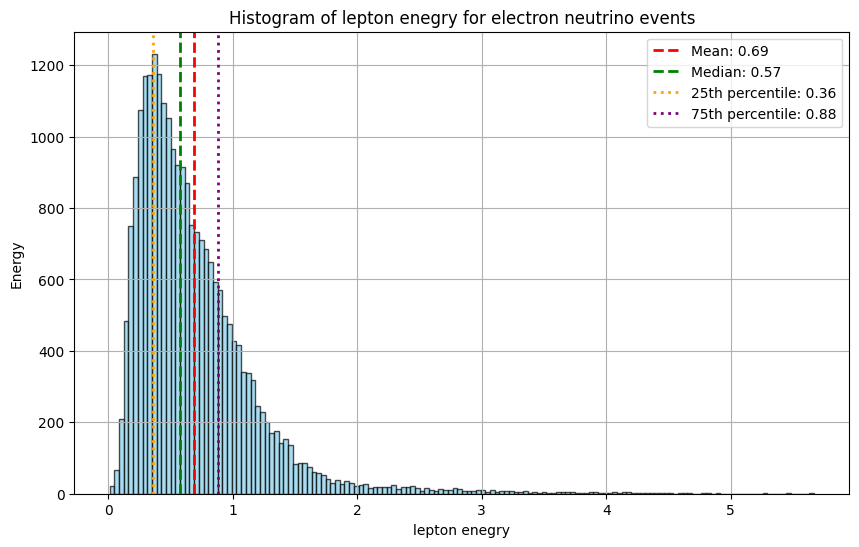
\includegraphics[width=0.95\textwidth]{src/leptonElectron.png}
        \caption{Lepton energy distribution in the \textbf{Inclusive} (BNB) sample. The vertical axis shows the number of events [count].}
        \label{fig:lepton-inclusive}
    \end{minipage}
    \hfill
    \begin{minipage}[t]{0.6\textwidth}
    \centering
    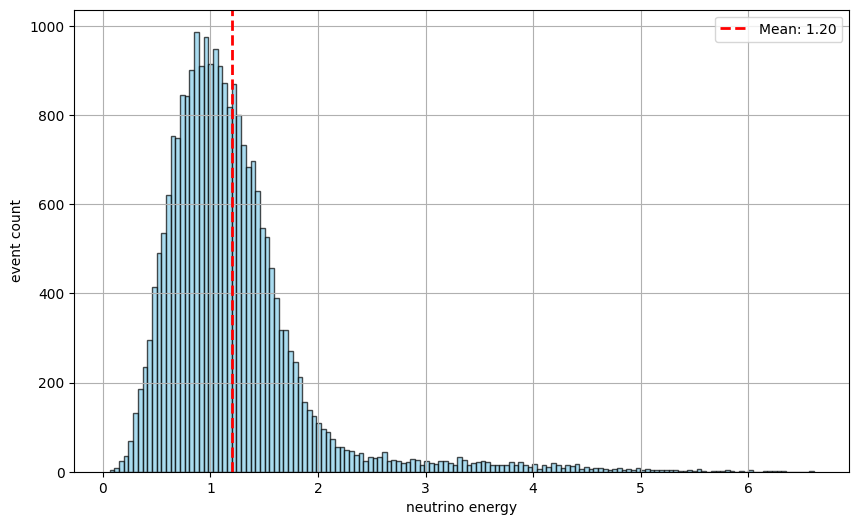
\includegraphics[width=0.95\textwidth]{src/neutrinoElectron.png}
    \caption{Neutrino energy distribution in the \textbf{Inclusive} (BNB) sample. The vertical axis shows the number of events [count].}
    \label{fig:neutrino-inclusive}
    \end{minipage}
\end{figure}

The BNB (Booster Neutrino Beam, Inclusive) sample contains a total of 24,332 events, all of which are classified as charged-current (CC) interactions. The dataset is composed exclusively of electron neutrinos and antineutrinos, with 19,448 events corresponding to neutrinos (PDG code 12) and 492 to antineutrinos (PDG code $-12$). No muon neutrinos (PDG 14 or $-14$) are present.

The energy distribution of neutrino interactions in this sample has a mean value of 1.62~GeV, a median of 1.46~GeV, and a standard deviation of 0.86~GeV. The minimum recorded energy is 0.13~GeV, while the maximum reaches 6.13~GeV.

The associated charged lepton energy distribution exhibits a mean of 0.69~GeV, a median of 0.57~GeV, and a standard deviation of 0.50~GeV. The lepton energies range from 0.01~GeV to 5.67~GeV. These characteristics reflect a relatively high-energy subset of interactions, with lepton energy distributions concentrated in the sub-GeV to low-GeV range.

\subsection{\texorpdfstring{$\nu_e$}{νₑ}-Enhanced Sample Description}

The distributions for the $\nu_e$-enhanced sample are shown in Figures~\ref{fig:lepton-nue} and~\ref{fig:neutrino-nue}.

\begin{figure}[H]
    \centering
    \begin{minipage}[t]{0.48\textwidth}
        \centering
        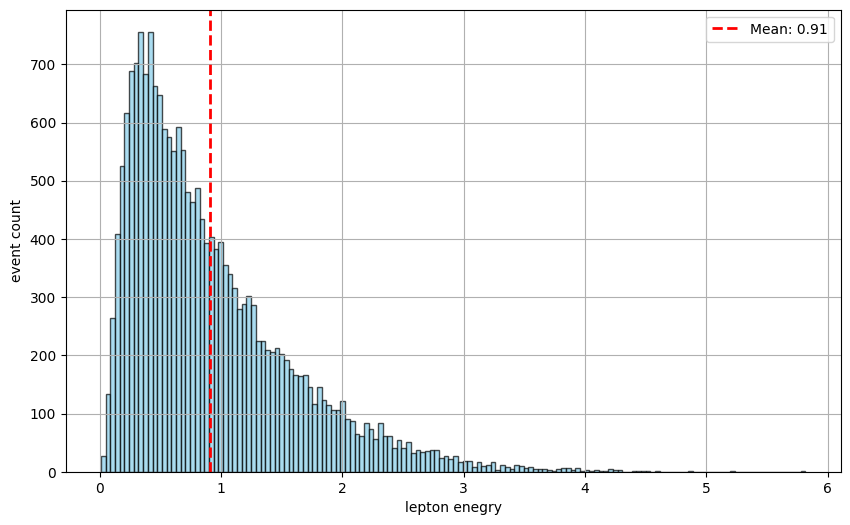
\includegraphics[width=0.8\textwidth]{src/leptonMuon.png}
        \caption{Lepton energy distribution in the \textbf{nu\_e}-enhanced sample. The vertical axis shows the number of events [count].}
        \label{fig:lepton-nue}
    \end{minipage}
    \hfill
    \begin{minipage}[t]{0.48\textwidth}
    \centering
    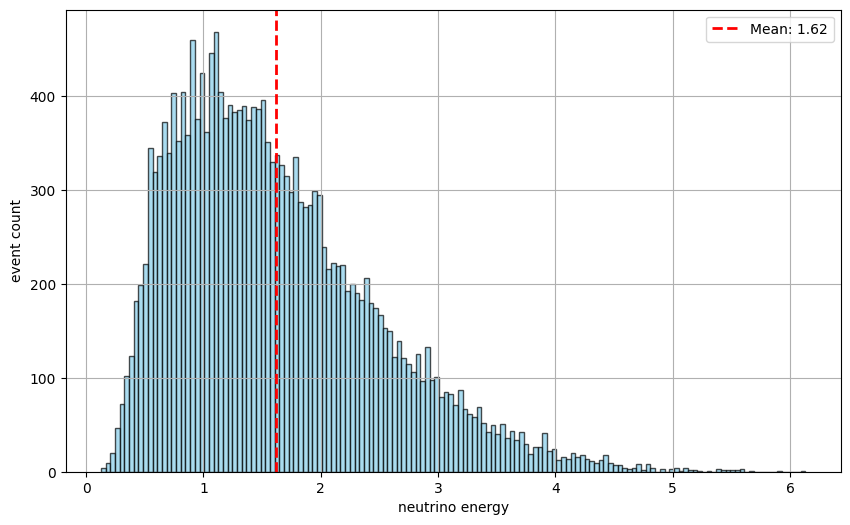
\includegraphics[width=0.8\textwidth]{src/neutrinoMuon.png}
    \caption{Neutrino energy distribution in the \textbf{nu\_e}-enhanced sample. The vertical axis shows the number of events [count].}
    \label{fig:neutrino-nue}
    \end{minipage}
\end{figure}

The $\nu_e$-enhanced sample consists of 19,940 events, containing a broader mix of neutrino types. The majority are muon neutrinos (23,984 with PDG code 14), followed by smaller numbers of muon antineutrinos (208 with PDG code $-14$), electron neutrinos (134 with PDG code 12), and electron antineutrinos (6 with PDG code $-12$). Of the total, 17,564 events are classified as charged-current (CC), while 6,768 are neutral-current (NC) interactions. Within the charged-current subset, 17,457 events originate from muon neutrinos or antineutrinos, and 107 from electron neutrinos or antineutrinos, indicating a dominance of muon neutrino interactions in this sample.

The energy distribution shows a mean of 1.20~GeV, a median of 1.08~GeV, and a standard deviation of 0.67~GeV, with values ranging from 0.06~GeV to 6.61~GeV. The corresponding charged lepton energy distribution has a mean of 0.91~GeV, a median of 0.73~GeV, and a standard deviation of 0.67~GeV. Lepton energies range from 0.01~GeV to 5.82~GeV. This distribution suggests a slightly lower-energy spectrum on average, but with a broader mix of interaction types and moderate lepton energy variability.

\begin{figure}[H]
    \centering
    \begin{minipage}[t]{0.48\textwidth}
        \centering
        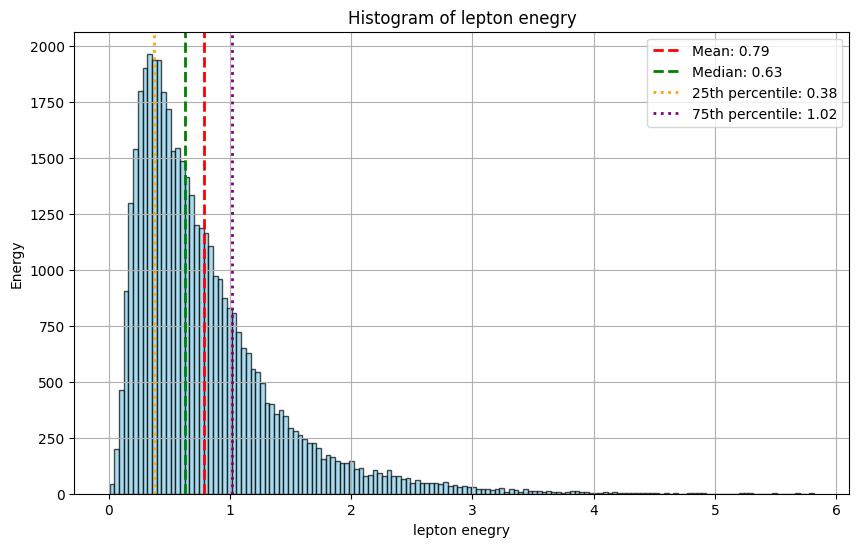
\includegraphics[width=0.8\textwidth]{src/leptonFull.png}
        \caption{Lepton energy distribution in the \textbf{Combined} dataset (Inclusive + nu\_e-enhanced). The vertical axis shows the number of events [count].}
        \label{fig:lepton-combined}
    \end{minipage}
    \hfill
    \begin{minipage}[t]{0.48\textwidth}
    \centering
    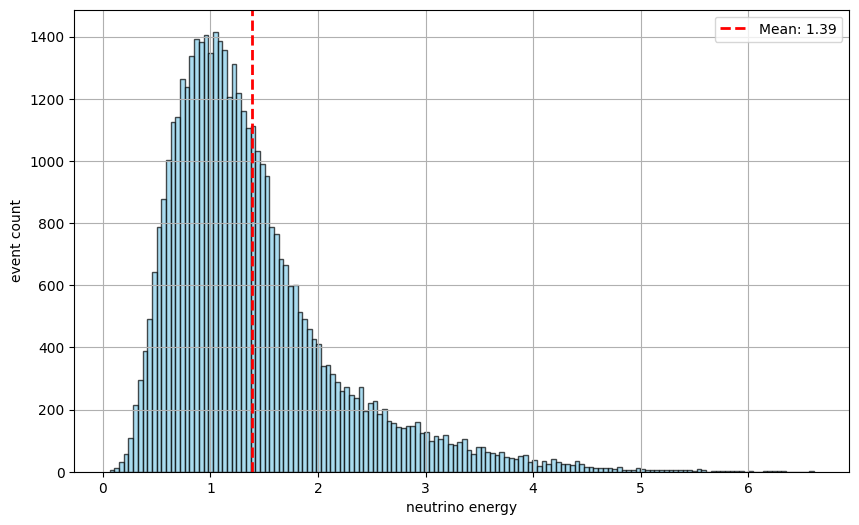
\includegraphics[width=0.8\textwidth]{src/neutrinoFull.png}
    \caption{Neutrino energy distribution in the \textbf{Combined} dataset (Inclusive + nu\_e-enhanced). The vertical axis shows the number of events [count].}
    \label{fig:neutrino-combined}
    \end{minipage}
\end{figure}

The combined dataset consists of 44,272 events and includes a mix of neutrino interaction types. The dominant component is muon neutrinos (23,984 events with PDG code 14), followed by electron neutrinos (19,582 with PDG 12), electron antineutrinos (498 with PDG $-12$), and a small number of muon antineutrinos (208 with PDG $-14$). Out of the total, 37,504 events are classified as charged-current (CC) interactions, while 6,768 are neutral-current (NC). Within the CC category, 17,457 events originate from muon neutrinos or antineutrinos, and 20,047 from electron neutrinos or antineutrinos, indicating a more balanced representation of flavor types compared to the $\nu_e$-enhanced sample. The charged lepton energy distribution exhibits a mean of 0.79~GeV, a median of 0.63~GeV, and a standard deviation of 0.60~GeV. The energy values range from 0.01~GeV to 5.82~GeV. This suggests a lower average energy compared to the $\nu_e$-enhanced sample, with a more symmetric distribution and substantial contributions from both muon and electron neutrino interactions.

% Example LaTeX table for the selected neutrino event statistics
\begin{table}[H]
\centering
\caption{Summary of Neutrino Events in the Dataset}
\begin{tabular}{|l|r|}
\hline
\textbf{Category} & \textbf{Count} \\
\hline
Total events & 44,272 \\
BNB sample & 24,332 \\
$\nu_e$-enhanced sample & 19,940 \\
\hline
\multicolumn{2}{|c|}{\textbf{In $\nu_e$-enhanced sample}} \\
\hline
$\nu_{\mu}$ ($\text{PDG}=14$) & 23,984 \\
$\bar{\nu}_{\mu}$ ($\text{PDG}=-14$) & 208 \\
$\nu_e$ ($\text{PDG}=12$) & 134 \\
$\bar{\nu}_e$ ($\text{PDG}=-12$) & 6 \\
Charged current (CC) events & 17,564 \\
Neutral current (NC) events & 6,768 \\
CC $\nu_e$ or $\bar{\nu}_e$ events & 107 \\
CC $\nu_e$ events & 101 \\
CC $\nu_{\mu}$ or $\bar{\nu}_{\mu}$ events & 17,457 \\
CC $\nu_{\mu}$ events & 17,338 \\
\hline
\multicolumn{2}{|c|}{\textbf{Energy statistics ($\nu_e$-enhanced sample)}} \\
\hline
Mean (GeV) & 1.20 \\
Median (GeV) & 1.08 \\
Std. deviation (GeV) & 0.67 \\
Min (GeV) & 0.06 \\
Max (GeV) & 6.61 \\
\hline
\multicolumn{2}{|c|}{\textbf{In BNB sample}} \\
\hline
$\nu_e$ ($\text{PDG}=12$) & 19,448 \\
$\bar{\nu}_e$ ($\text{PDG}=-12$) & 492 \\
CC events & 19,940 \\
CC $\nu_e$ or $\bar{\nu}_e$ events & 19,940 \\
CC $\nu_e$ events & 19,448 \\
CC $\nu_{\mu}$ or $\bar{\nu}_{\mu}$ events & 0 \\
\hline
\multicolumn{2}{|c|}{\textbf{Energy statistics (BNB sample)}} \\
\hline
Mean (GeV) & 1.62 \\
Median (GeV) & 1.46 \\
Std. deviation (GeV) & 0.86 \\
Min (GeV) & 0.13 \\
Max (GeV) & 6.13 \\
\hline
\end{tabular}
\end{table}

\section{Environment Preparation}

The Jupyter notebooks accompanying the MicroBooNE OpenSamples repository recommend creating a Conda environment that includes the necessary packages. While there is nothing inherently wrong with this approach, it does introduce several disadvantages. Beyond general inefficiencies—such as longer environment loading times, higher memory usage, and increased disk space consumption—the most significant issue encountered was related to the sheer number of files generated by Conda distributions.

Both Conda and Miniconda installations can create and maintain hundreds of thousands of files. Although the total disk usage of these files is typically not problematic (many are symbolic links or small metadata files), the system used for processing data enforced strict quotas on the number of files each user could create. The data processing was performed on the ICM UW Okeanos cluster running CentOS 7{SPRAWDZIĆ}. Installing a full Conda distribution brought the user account dangerously close to this limit, which severely impacted the usability of the system. For instance, launching a new Jupyter session became almost impossible, as nearly every action related to managing Jupyter generates additional log files, further pushing against the file quota.

Additionally, the environment setup proposed in the MicroBooNE OpenSamples notebooks depended on outdated libraries—most notably \texttt{pynuml} version 0.3, which is no longer maintained and is poorly documented. This package also requires an outdated version of Python (3.7) and depends on a deprecated version of HDF5. These constraints make it effectively impossible to use current versions of many essential packages, which significantly complicates the development process.

To address these issues and improve the portability and maintainability of the tools used for processing OpenSamples data, an alternative approach to environment management was adopted.

\subsection{Containerization and Singularity}

Containerization is a method of packaging software and its dependencies into isolated, self-contained units called containers. Each container includes all necessary binaries, libraries, and configuration files, ensuring that applications run consistently across different systems regardless of variations in the underlying infrastructure. Modern containerization solutions allow for building, distributing, and executing containers in a lightweight and reproducible manner. Containers are typically defined using a configuration file that builds on a base image and specifies additional dependencies and setup steps, producing a new image that can be versioned and reused.

In this specific case, a containerization tool called Singularity was used. Singularity is particularly well-suited for high-performance computing environments, as it enables users to define, build, and execute containers without requiring root privileges. A container definition file was created based on a Ubuntu 22.01 base image. (An image is a static, read-only template with the application and its dependencies, while a container is a running instance of an image, including its own filesystem and processes.) This definition specified the installation of all required dependencies and packages during the container build process. Using this approach made it possible to work with up-to-date software versions, including Python 3.9, pynuml version 25.4.0, and HDF5 version 1.12.2, although these upgrades required some code refactorings to be performed on the code present in OpenSamples notebooks. Moreover, since the resulting container image is stored as a single file, this method also effectively circumvented the file quota limitations encountered with Conda-based setups.

\section{Dataset Preparation}

\subsection{HDF5 File Structure}

Data stored in HDF5 files was separated into multiple tables, each containing a specific type of information. The tables are organized hierarchically, with the root directory containing the main event table and additional subdirectories for other data types. Each table is structured as a collection of records, where each record corresponds to a single event or hit in the detector. The tables are designed to be self-describing, meaning that they include metadata about the data types and structures used within them.
The HDF5 file structure for the MicroBooNE OpenSamples dataset is organized as follows:

\begin{table}[H]
\centering
\begin{tabular}{|l|p{10.5cm}|}
\hline
\textbf{Table Name} & \textbf{Description} \\
\hline
\texttt{/event\_table} & Stores metadata for individual detector readouts and simulated neutrino interactions. Includes event identifiers, neutrino properties (energy, direction), interaction vertex, and interaction type (charged- or neutral-current). \\
\hline
\texttt{/hit\_table} & Contains reconstructed hits from Gaussian pulses on wire waveforms. Includes hit positions, times, plane/wire IDs, and signal properties like integral and RMS. \\
\hline
\texttt{/edep\_table} & Holds simulated true energy deposition data within the TPC. Entries link to the associated hit and originating simulated particle. \\
\hline
\texttt{/particle\_table} & Stores detailed simulation data for particles from neutrino interactions as simulated by Geant4, including start/end positions, momenta, parent-child relationships, and process labels. \\
\hline
\texttt{/opflash\_table} & Contains reconstructed optical flash data detected by PMTs, such as time, width, and spatial barycenter. \\
\hline
\texttt{/opflashsumpe\_table} & Provides total photoelectron (PE) counts per PMT for each optical flash, useful for calibrated optical signal reconstruction. \\
\hline
\texttt{/ophit\_table} & Details individual PMT hits, including amplitude, width, time, and associated PMT channel. Links to flash and PE sum tables. \\
\hline
\texttt{/pandoraHit\_table} & Describes how individual TPC hits are grouped into clusters by the Pandora reconstruction framework. Includes associations to PFParticles and time slices. \\
\hline
\texttt{/pandoraPfp\_table} & Stores data for Pandora-reconstructed PFParticles, which represent 3D hit clusters. Contains particle type IDs, vertex info, and classification scores. \\
\hline
\texttt{/pandoraPrimary\_table} & Contains metadata for interactions (primaries) identified by Pandora, including neutrino/cosmic classification scores and optical-TPC flash matching quality. \\
\hline
\texttt{/wire\_table} & Records full waveform data for each detector wire over 6400 time ticks. Provides raw ADC values for hit reconstruction. Only in ``With Wire'' datasets. \\
\hline
\end{tabular}
\caption{Summary of tables and their contents in the detector data model.}
\label{tab:data_tables}
\end{table}


\subsection{Final dataset structure}

Because of their smaller size, HDF5 files were used for the initial data extraction. Although the HDF5 format is well-suited for storing large datasets, reading from it can require loading substantial portions of data into memory—a time-consuming operation that makes it impractical to use these files directly for neural network training. Therefore, a decision was made to extract the relevant data and store it in a simpler, more accessible format.

The final extracted dataset consisted of a CSV file containing the composite event ID (run number, subrun number, and event number), the lepton energy, neutrino energy, and the \texttt{is\_cc} value from the event table, as well as the \texttt{PDG} of the interacting neutrino. Additionally, it included the filenames of three image files, each corresponding to one of the three wire planes. These images were generated from the wire readouts and represent visualizations of the recorded signals.

\subsection{General data extraction}

Data from the \texttt{wire\_table}, \texttt{edep\_table}, and \texttt{lep\_table} were first matched with corresponding events in the \texttt{event\_table} (this was largely based on the code present in the Wireimage.ipynb notebook provided by the authors of the dataset). From each matched record, the lepton energy was extracted from the \texttt{lep\_table}, the neutrino energy from the \texttt{edep\_table}, and the \texttt{is\_cc} value from the \texttt{event\_table}. The \texttt{wire\_table} was used to obtain the wire signals for each event. It was subsequently processed into images, and linked to the corresponding event metadata for downstream analysis.

\section{Image Rendering}

\begin{figure}[H]
    \centering
    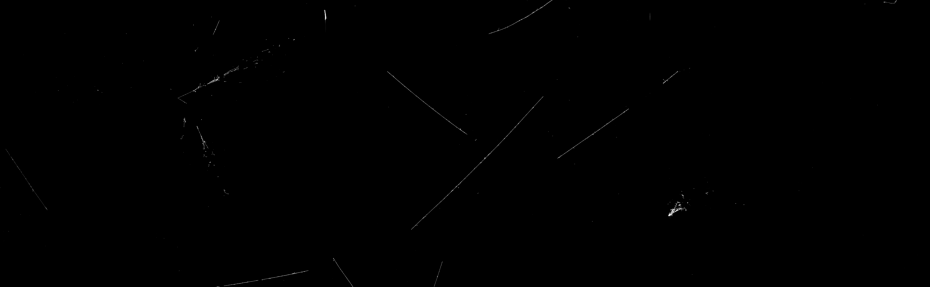
\includegraphics[width=0.7\textwidth]{src/with_flag_58.png}
    \caption{Example of a wire readout image}
\end{figure}


Images were generated using data from the wire readouts, where the horizontal axis corresponds to the wire number and the vertical axis to time. Each pixel represents the signal recorded on a specific wire at a given time. To suppress noise, a threshold was applied, below which wire activity was not visualized. Additionally, a saturation limit was introduced to prevent high-intensity signals from dominating the image. Pixel intensities were linearly scaled to an 8-bit range (0--255), and the resulting images were downsampled by a factor of two to reduce dataset size. This procedure was applied to all three wire planes, producing three images per event. These images were later saved as PNG files, and their filenames were stored in an appropriate CSV manifest file (a summary file listing all images and their associated metadata for each event).

\subsection{Final Dataset}

The final dataset consisted 132,816 PNG images, each representing a wire readout from the MicroBooNE detector alongside 38 CSV manifest files, each representing events form a single HDF5 file. This dataset turend out to contain approximately 13~GB of data, with each image file averaging around 100~KB in size.

\section{Further Dataset Processing}

Although the final image dataset occupied approximately 13~GB on disk, this was primarily due to the use of compressed image formats (specifically, PNG). When these images were loaded into memory as arrays of integers, their size increased dramatically—by more than a factor of 100 in some cases. It quickly became evident that the dataset was too large to be feasibly loaded into the system's RAM without causing memory fragmentation. However, loading each image individually into memory incurred significant computational overhead: each image had to be read from disk, memory had to be allocated, and the image had to be decompressed before being converted into an array. Since training a convolutional neural network (CNN) typically requires each image to be loaded multiple times, it was crucial to minimize the number of image loading operations.

\begin{figure}[H]
    \centering
    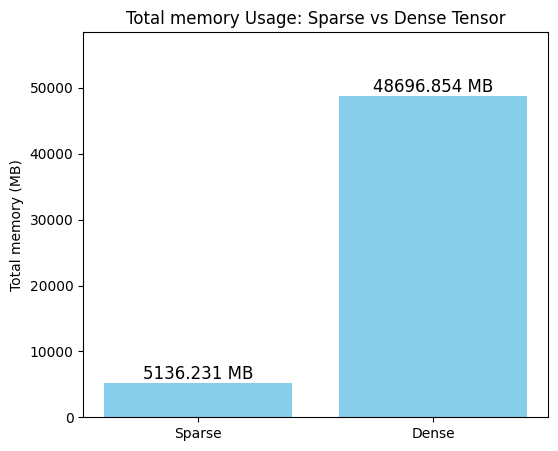
\includegraphics[width=0.7\textwidth]{src/totalSparseDense.png}
    \caption{Comparison of total memory usage between dense and sparse array representations.}
\end{figure}

During development, it was observed that the processed images contained mostly empty (zero-value) pixels. While tracks were present in all images, they typically occupied only a small portion of each image—approximately 5\% of the total pixels. (Note: Mention that the threshold used during the generation of wire images was sufficiently low to eliminate noise.) As a result, the decision was made to represent the images using sparse arrays (implemented with \texttt{torch.sparse}).... Unlike dense arrays, where each element is stored explicitly in memory, sparse arrays assume a default value for all positions and store only the non-zero values along with their coordinates. Although these sparse arrays still need to be converted to dense format before being passed to the CNN, this conversion is significantly less costly than loading and decompressing images from disk. This optimization led to a substantial reduction in memory usage—by up to a factor of 70—making it feasible to load the entire dataset into RAM.

\begin{figure}[H]
    \centering
    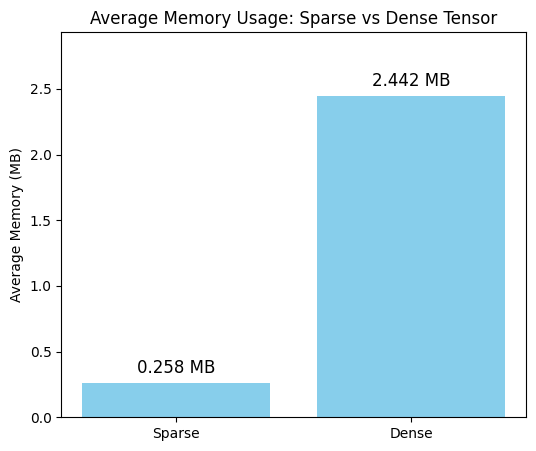
\includegraphics[width=0.7\textwidth]{src/sparseDenseComp.png}
    \caption{Comparison of average memory usage between dense and sparse array representations.}
\end{figure}

Another challenge arose from the number of individual files comprising the dataset. The final dataset contained approximately 120,000 image files. This created issues similar to those previously encountered when working with Miniconda—namely, the operaing system configurations used on ICM rysy and topola clusters used for CNN training imposed quotas on the number of files each user could allocate. Operating under an account close to that limit proved to be cumbersome. Notably, the total dataset size remained well below the storage quota in terms of bytes, indicating that reducing the number of files could resolve the problem without affecting overall storage usage.

To address both issues, each CSV manifest file was loaded into a pandas DataFrame. Three additional columns were added to each record—one for each image associated with an event—and populated with the corresponding sparse arrays. Each resulting dataset was then saved as a single \texttt{.pkl} file, a format that preserves Python objects as they exist in memory. In total, 38 .pkl files were created, each corresponding to one original HDF5 file and containing all events and associated images from that file. The combined size of all \texttt{.pkl} files was approximately 32~GB, which corresponds closely to the amount of memory required to load them into RAM.

\section{Classification Task and Data Selection}


POPRAWIĆ
The classification task is to distinguish electron neutrino charged current (CC) interactions from all other events based on the wire readout images.

To simplify the initial stages of analysis, the decision was made to focus on the most straightforward and visually distinct case: electron neutrino charged current (CC) interactions. These interactions produce energetic electrons that initiate electromagnetic showers, which leave highly visible and easily identifiable traces in the detector. Based on this, the dataset was divided into two classes—electron neutrino CC interactions and all other types of events. It was further hypothesized that higher-energy neutrinos are likely to produce more energetic electrons, which in turn generate more pronounced and spatially extended showers. Such events are presumed to be easier to detect and classify reliably. To leverage this property, the dataset was further narrowed down by selecting the top 50\% most energetic electron neutrino CC events, thereby prioritizing those cases with the clearest and most informative signatures.

\section{Machine Learning}

Machine learning algorithms aim to find a mapping from a specific set of points in an input space to a corresponding set of points in an output space, both of which are predefined. These algorithms define a procedure for learning such a mapping based on a given set of input-output pairs, commonly referred to as the training data. Once learned, this mapping can be applied to all points in the input space, including those not included in the training set. The general expectation is that the mapping learned from the training data will generalize well to previously unseen data, enabling the algorithm to make accurate predictions or classifications on new inputs.

\subsection{supervised machine learning}

The problems tackled in this work are classification problems, where the input space consists of images of wire readouts, and the output space consists of a binary label. The common way of tackling such problems is supervised machine learning.
In supervised machine learning, the training data is given in the form of input-target pairs \( \{(\mathbf{x}_i, y_i)\}_{i=1}^N \), where \( \mathbf{x}_i \in \mathbb{R}^d \) represents the feature vector of the \( i \)-th input and \( y_i \in \mathcal{Y} \) is the corresponding target value. The aim is to learn a function \( f: \mathbb{R}^d \rightarrow \mathcal{Y} \) that approximates the true relationship between inputs and outputs.

The central objective is to find a function \( f \) such that:
\[
f(\mathbf{x}_i) \approx y_i \quad \forall i \in \{1, \dots, N\}
\]

\subsection{Machine learning model and learnable Parameters}

The term machine learning model mentioned futrher in the work will refer to a pairing of a set of learnable parameters \( \boldsymbol{\theta} \in \mathbb{R}^p \), where \( p \) is the total number of parameters, and a model function \( f(\mathbf{x}; \boldsymbol{\theta}) \) which maps the input space to the output space. The learnable parameters \( \boldsymbol{\theta} \) are variables within the model that can be adjusted during the training process to minimize the difference between the model's predictions and the actual target values. They have a direct influence on the model's output.


The training process begins by setting all elements of \( \boldsymbol{\theta} \) with some initial values. For each training iteration, a batch of input data \( \mathbf{X} \in \mathbb{R}^{b \times d} \) is passed through the model, and the corresponding predictions \( \hat{\mathbf{y}} \in \mathbb{R}^b \) are obtained:

\[
\hat{\mathbf{y}} = f(\mathbf{X}; \boldsymbol{\theta})
\]

These predictions are then compared to the true labels \( \mathbf{y} \in \mathbb{R}^b \), and the parameters \( \boldsymbol{\theta} \) are updated to reduce the discrepancy. This step is repeated iteratively, refining \( \boldsymbol{\theta} \) over time to improve predictive performance. Each such update constitutes a learning step, and the entire iterative process is referred to as model training.

\subsection{Loss Function}

The quality of the model's predictions is assessed using a loss function 

\[
\( \mathcal{L}(\hat{y}, y) \)
\]

Here $y$ stands for the true target value, while \( \hat{y} = f(\mathbf{x}; \boldsymbol{\theta}) \) is the model's prediction for a given input \( \mathbf{x} \).

The role of this function is to quantify the difference between predicted and true outputs. By assumtion the value of the loss function is non-negative, with lower values indicating better model performance (the outputs of the model are given ).

The choice of an optimal loss function is problem-specific but, regardless of the choice, the goal is to minimize the loss function with respect to the model parameters:

\[
\min_{\boldsymbol{\theta}} \ \mathcal{L}(f(\mathbf{x}; \boldsymbol{\theta}), y)
\]

\subsection{Cross-Entropy Loss}

Because of the nature of the problems discussed in this work, the cross-entropy loss function was used. This loss function is commonly applied to classification tasks.

The function in question measures the dissimilarity between the predicted probability distribution \( \hat{\mathbf{y}} \) over classes and the true class label distribution \( \mathbf{y} \), typically represented as a \textit{one-hot encoded vector}—a binary vector of length \( C \), where all entries are zero except for a one at the index corresponding to the correct class. For a single example and \( C \) classes, the cross-entropy loss is defined as:
\[
\mathcal{L}_{\text{CE}}(\mathbf{y}, \hat{\mathbf{y}}) = -\sum_{i=1}^{C} y_i \log(\hat{y}_i)
\]

This loss penalizes incorrect confident predictions more heavily and encourages the model to assign high probability to the correct class. Minimizing the cross-entropy therefore drives the model to output probability distributions that closely align with the true labels.

\subsection{Gradient Descent Optimization}

\begin{figure}[H]
    \centering
    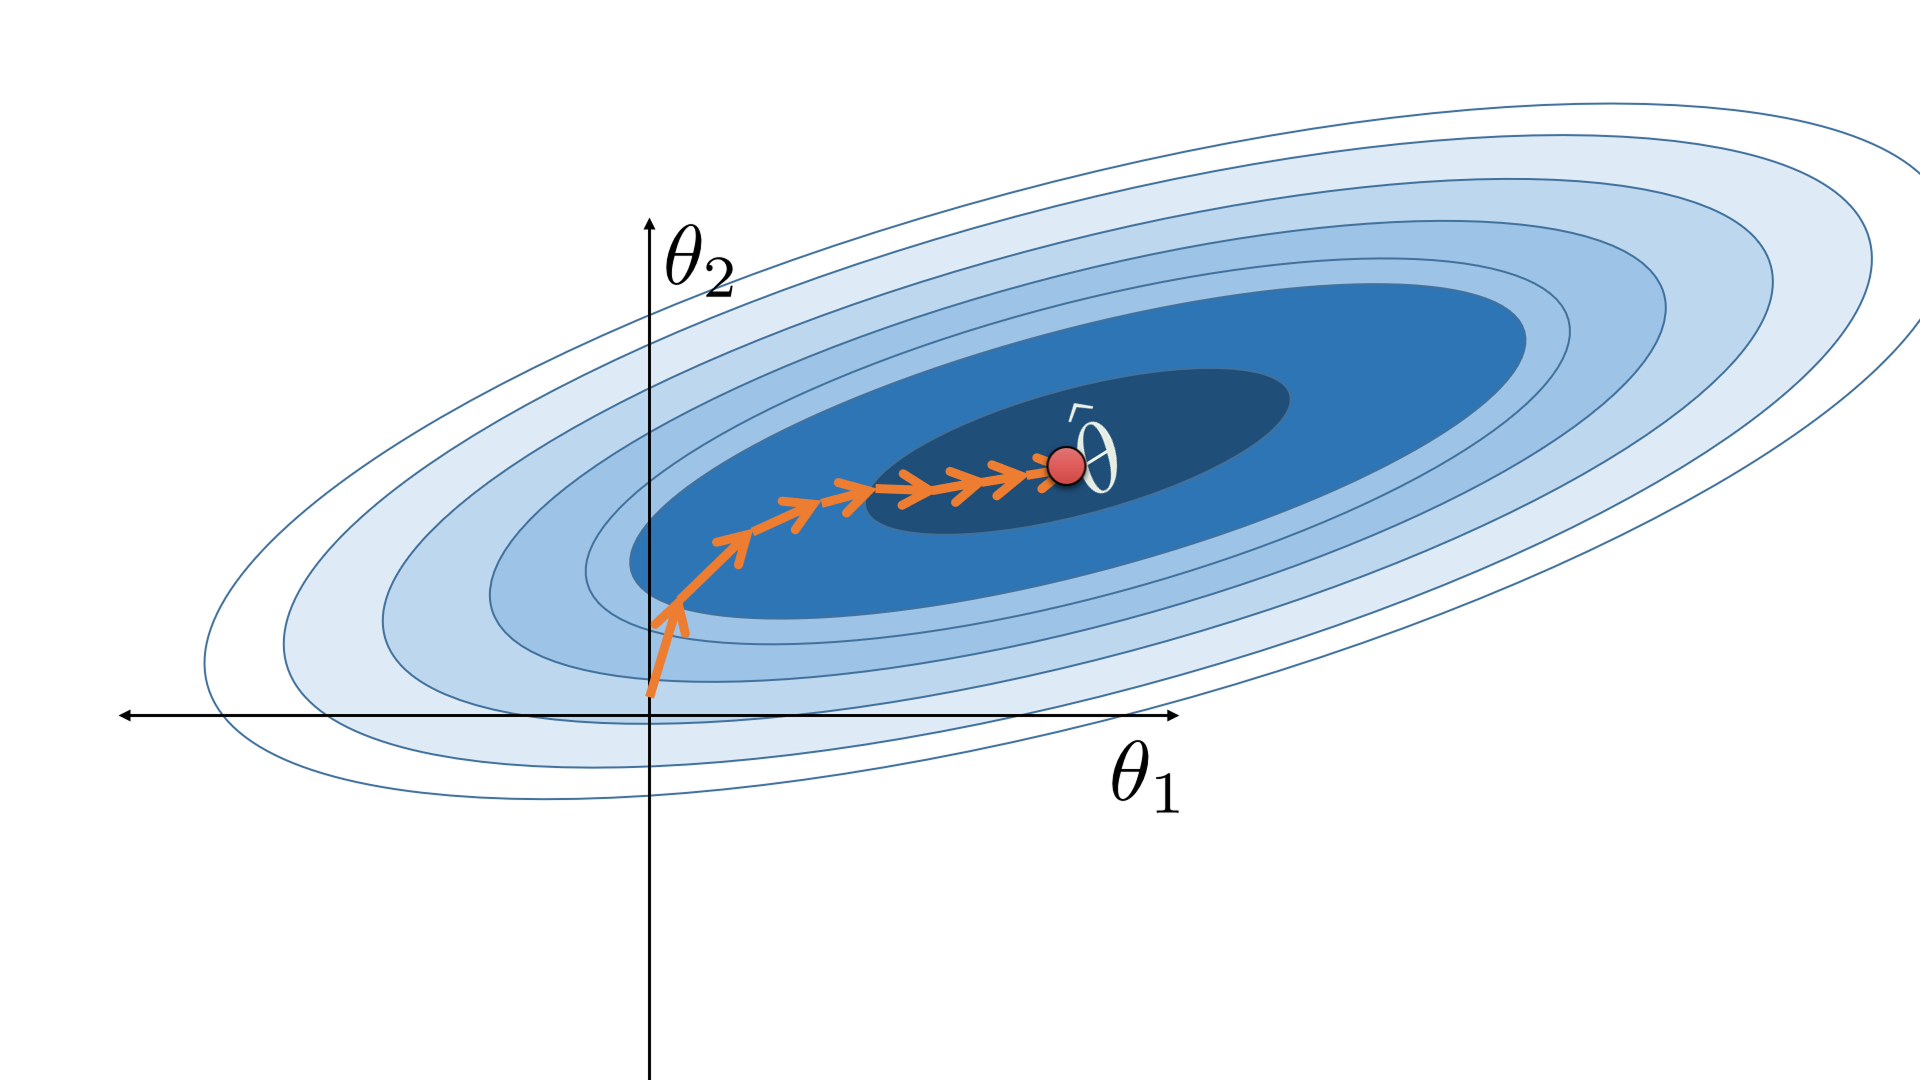
\includegraphics[width=0.85\textwidth]{src/gradienDescent.png}
    \caption{Gradient descent visualization. A local minimum is achieved by taking steps of a predefined size in the direction of the steepest descent.}
\end{figure}

The approach used for training models used in this work is called \textit{gradient descent}. In particular, stochastic gradient descent (SGD). In each iteration, the gradient of the loss function with respect to the model parameters is computed:

\[
\nabla_{\boldsymbol{\theta}} \mathcal{L} = \left[ \frac{\partial \mathcal{L}}{\partial \theta_1}, \frac{\partial \mathcal{L}}{\partial \theta_2}, \dots, \frac{\partial \mathcal{L}}{\partial \theta_p} \right]^\top
\]

This gradient vector indicates the direction in parameter space that increases the loss most steeply. The parameters are then updated in the opposite direction of the gradient to reduce the loss:

\[
\boldsymbol{\theta} \leftarrow \boldsymbol{\theta} - \eta \nabla_{\boldsymbol{\theta}} \mathcal{L}
\]
where \( \eta > 0 \) is the learning rate, a hyperparameter that controls the step size.

By repeating this process over multiple iterations and batches of training data, the parameters ideally converge to a local minimum of the loss function. At convergence, the model's predictions are as close as possible to the target values within the expressiveness of the chosen architecture.

This iterative process of computing gradients and updating parameters is known as \textit{gradient descent}.

\subsubsection{Momentum}

In order to smooth out the gradient descent and accelerate convergence a \textit{momentum} can be introduced to a sdg algorithm. When introduced the descent direction incorporates a fraction of the previous update step, instead of relying solely on the current gradient.

The momentum update rule is defined as:

\[
\begin{aligned}
\mathbf{v}_t &= \gamma \mathbf{v}_{t-1} + \eta \nabla_{\boldsymbol{\theta}} \mathcal{L}(\boldsymbol{\theta}_{t-1}) \\
\boldsymbol{\theta}_t &= \boldsymbol{\theta}_{t-1} - \mathbf{v}_t
\end{aligned}
\]

Here, \( \mathbf{v}_t \) is the velocity vector (accumulated update), \( \gamma \in [0,1) \) is the momentum coefficient, and \( \eta \) is the learning rate. A higher \( \gamma \) allows more influence from previous gradients, leading to smoother and potentially faster convergence.


\section{Performance Metrics}

To evaluate the performance of the trained classification models, several metrics were used. These metrics provide complementary insights into different aspects of classification performance, especially in the context of imbalanced data.

\subsection{F1 Score}

The F1 score is the harmonic mean of precision and recall, offering a balanced measure that accounts for both false positives and false negatives. For a binary classification problem, precision and recall are defined as:

\[
\text{Precision} = \frac{\text{TP}}{\text{TP} + \text{FP}}, \quad
\text{Recall} = \frac{\text{TP}}{\text{TP} + \text{FN}}
\]

where TP, FP, and FN denote true positives, false positives, and false negatives, respectively. The F1 score is then given by:

\[
F_1 = 2 \cdot \frac{\text{Precision} \cdot \text{Recall}}{\text{Precision} + \text{Recall}}
\]

A higher F1 score indicates better performance, particularly when precision and recall are both high. These metrics are especially relevant when class distribution is skewed or when the cost of false positives and false negatives differs.

\subsection{Confusion Matrix}

The confusion matrix is a tabular summary of classification results. It displays the counts of true positive (TP), false positive (FP), true negative (TN), and false negative (FN) predictions. For a binary classification problem, the confusion matrix is a 2×2 matrix of the form:

\[
\begin{bmatrix}
\text{TP} & \text{FN} \\
\text{FP} & \text{TN}
\end{bmatrix}
\]

Each cell corresponds to a specific prediction outcome. From this matrix, additional metrics can be derived. For example, \textit{specificity} measures the true negative rate:

\[
\text{Specificity} = \frac{\text{TN}}{\text{TN} + \text{FP}}
\]

Normalizing the matrix enables interpretation in terms of proportions, helping to identify potential biases in the model's predictions.

\subsection{ROC Curve and AUC}

The Receiver Operating Characteristic (ROC) curve illustrates the diagnostic ability of a classifier as its decision threshold is varied. It plots the true positive rate (TPR) against the false positive rate (FPR):

\[
\text{TPR} = \frac{\text{TP}}{\text{TP} + \text{FN}}, \quad
\text{FPR} = \frac{\text{FP}}{\text{FP} + \text{TN}}
\]

The Area Under the Curve (AUC) summarizes the ROC curve in a single scalar value between 0 and 1. An AUC of 0.5 indicates random guessing, while an AUC of 1.0 represents perfect classification.

\section{Convolutional Neural Networks (CNNs)}

% \textit{Source:} \url{file:///C:/Users/wojte/Downloads/s13244-018-0639-9.pdf}

Convolutional neural networks (CNNs) are a class of machine learning algorithms designed to automatically and adaptively learn spatial hierarchies of features, ranging from low-level edges to high-level semantic patterns. They consist of stacked convolutional and pooling layers responsible for feature extraction, followed by fully connected layers that perform the final classification. Each layer passes its output to the next, enabling progressively more abstract and complex features to be learned as information flows through the network.

\subsection{Convolutional Layer}

\begin{figure}[H]
    \centering
    \begin{minipage}[t]{0.48\textwidth}
        \centering
        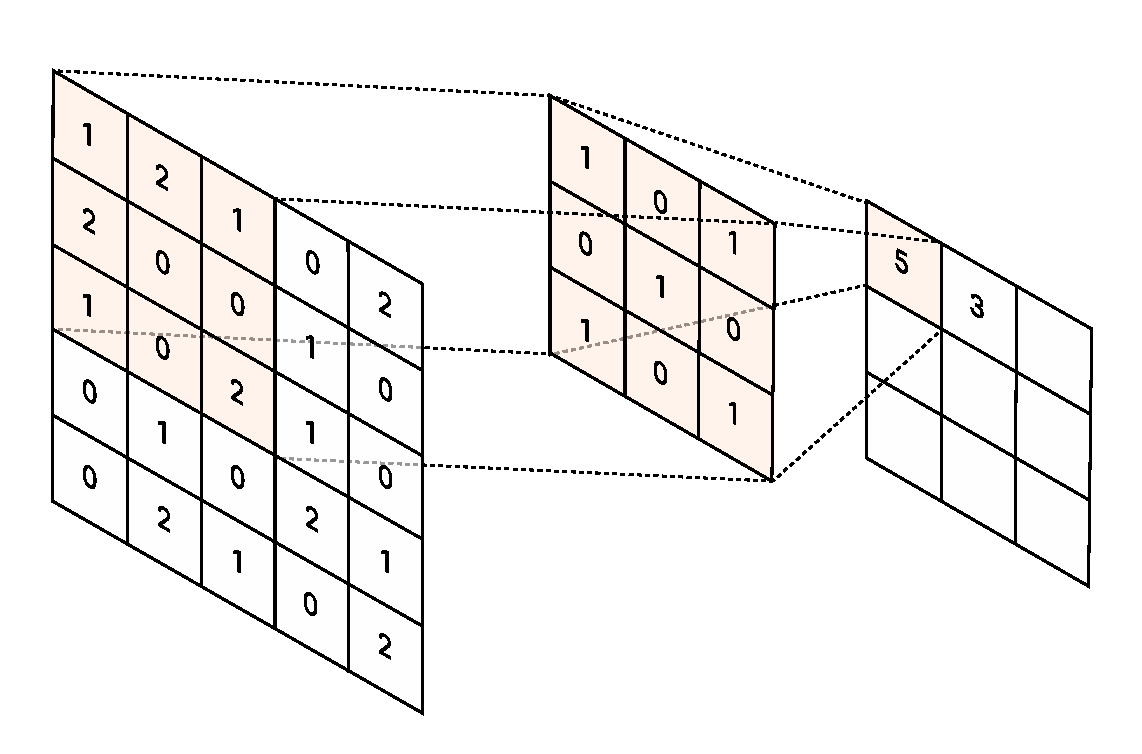
\includegraphics[width=\textwidth]{src/conv1.pdf}
        \caption{Caption for conv1.pdf}
    \end{minipage}
    \hfill
    \begin{minipage}[t]{0.48\textwidth}
        \centering
        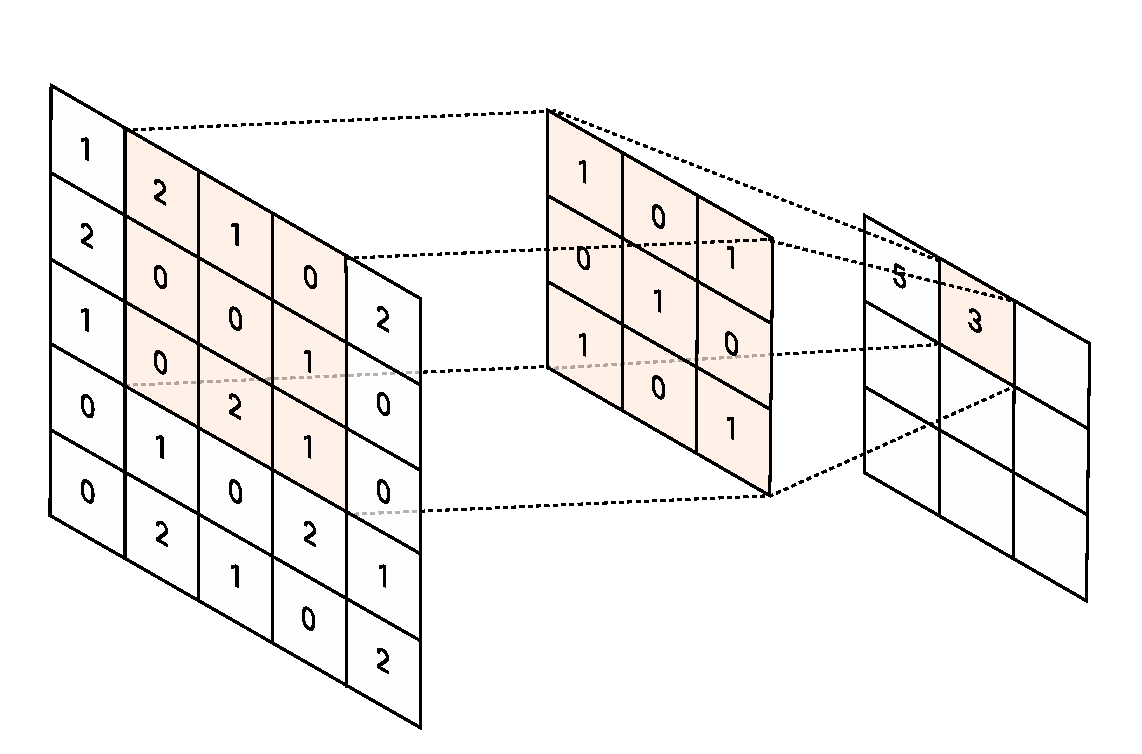
\includegraphics[width=\textwidth]{src/conv2.pdf}
        \caption{Caption for conv2.pdf}
    \end{minipage}
\end{figure}

\subsubsection{General Mechanism}

A convolution is a linear operation that involves element-wise multiplication between an input array and a corresponding kernel (also referred to as a \textit{filter}), followed by summation of the resulting products. The kernel is an array of values, typically smaller than the input array, that defines the operation and characterizes the specific features being extracted.

In a convolutional layer, multiple such kernels are applied to every valid subsection of the input array with dimensions matching the kernel size. The result of each convolution is a single scalar value, which becomes an element of the output feature map. To preserve or control the spatial dimensions of the output, \textit{padding} may be applied to the input array, typically by adding zeros around its border.

The output of a convolutional layer is an array (or tensor) with reduced spatial dimensions (depending on the padding and stride) and a number of channels equal to the number of kernels employed in the layer.

\subsubsection{Feature Recognition Mechanism}

\begin{figure}[H]
    \centering
    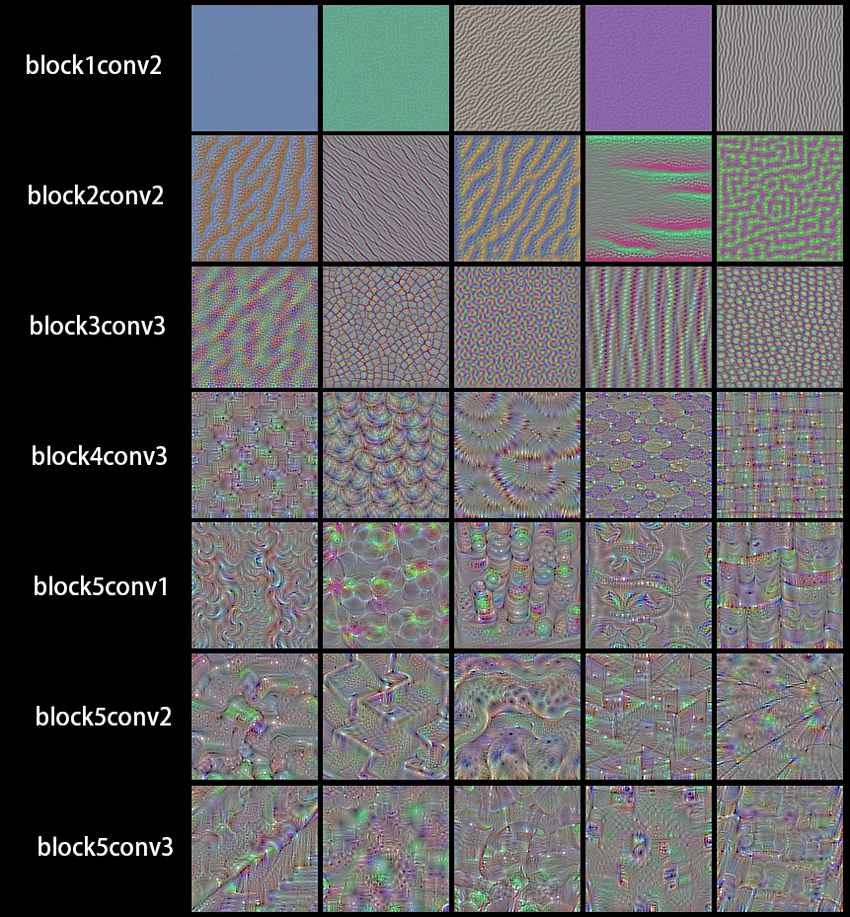
\includegraphics[width=0.5\textwidth]{src/convViz.png}
    \caption{Visualization of convolution operation (convViz.png) {ADD EXPLENATION}\cite{exCNN}}
\end{figure}

During backpropagation, each element of every kernel is treated as a learnable parameter and is optimized using gradient descent. The gradients of these parameters are computed with respect to each input element (more precisely, with respect to each considered subsection of the input array). These gradients are then aggregated—typically by averaging—and the kernel parameters are updated accordingly.

The general objective is for the kernels to adjust themselves to specific features of the input image—that is, to produce high activation values when a particular feature is present and low values when it is absent. The calculated gradients for each subsection of the input array depend on the values of the inputs. Consequently, it is assumed that during training, the elements of the kernels are updated in such a way that each kernel learns to recognize a distinct feature in the input array.

\subsection{Pooling Layer}

\begin{figure}[H]
    \centering
    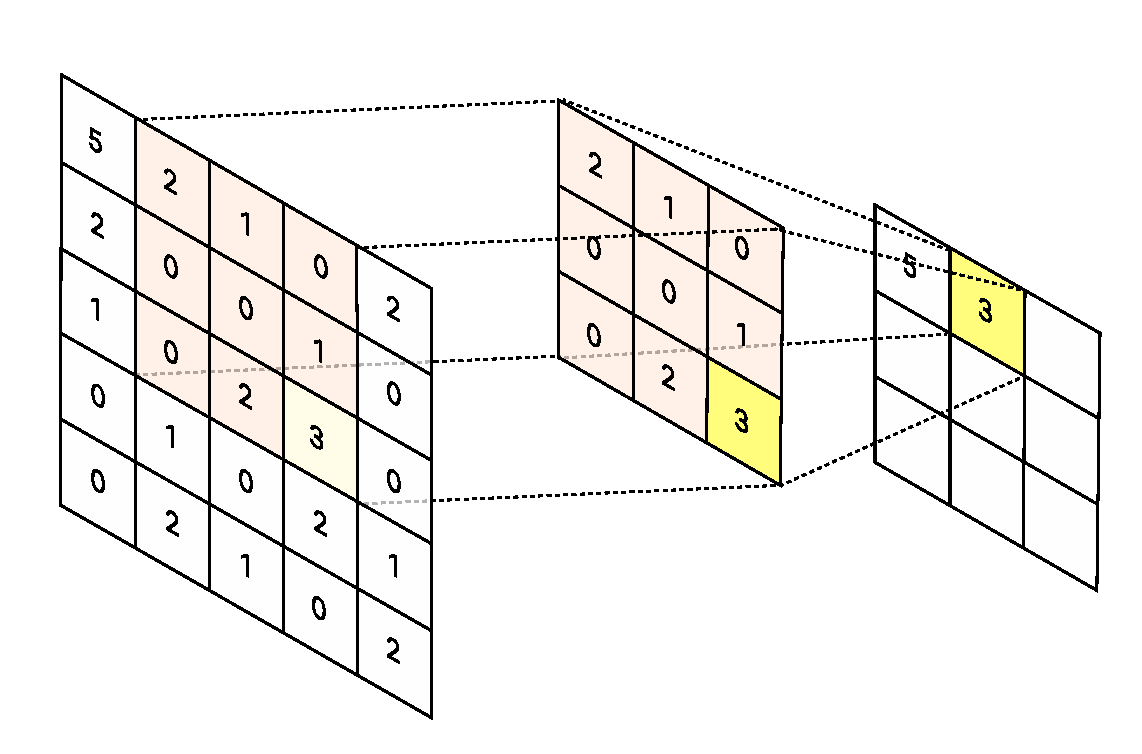
\includegraphics[width=0.8\textwidth]{src/pool1.pdf}
    \caption{Caption for conv2.pdf}
\end{figure}

A pooling layer is a downsampling operation used to reduce the spatial dimensions of feature maps while preserving salient information. The specific pooling method used in each layer is selected based on its effectiveness for the given classification task, typically determined through empirical evaluation. Among the available techniques, \textit{max pooling}—which selects the maximum value within a specified region—is the most commonly employed approach.

Pooling layers operate independently on each feature map (channel), where a channel corresponds to a set of activations produced by a single convolutional filter, and do not involve learnable parameters. By summarizing local regions, they can ensure invariance to small translations and reduce computational complexity in subsequent layers. Similar to convolutional layers, padding and stride can be used to control the spatial dimensions of the output.

\subsection{Multi-Layer Perceptron}

% TODO

\begin{figure}[H]
\centering
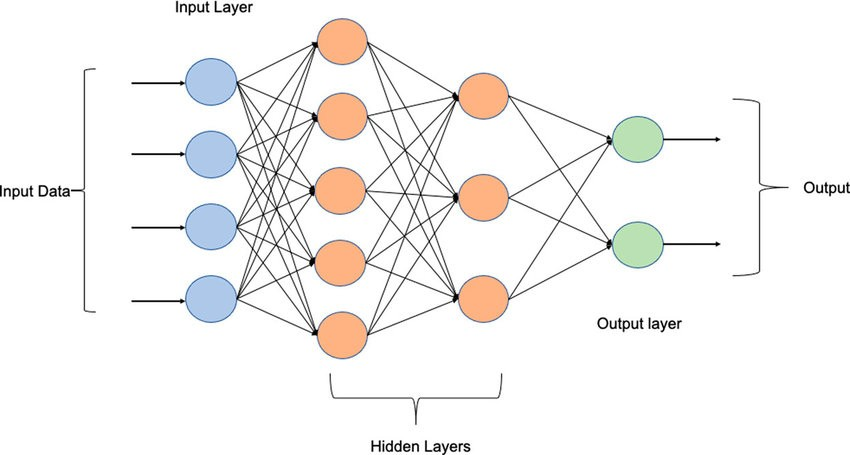
\includegraphics[width=0.6\textwidth]{src/mlp.jpg}
\caption{Illustration of a multi-layer perceptron architecture}
\end{figure}

A multi-layer perceptron (MLP) is a feed-forward neural network composed of multiple fully connected layers (ie. a layer where each neuron receives input from every neuron in the previous layer). The MLP used in this context typically consists of several layers with progressively smaller numbers of neurons, culminating in an output layer tailored to the classification task.

In classical CNN architectures, the output of the final convolution or pooling layer is flattened and passed into a multi-layer perceptron to perform the final classification.

\subsection{Complete CNN}

\begin{figure}[H]
    \centering
    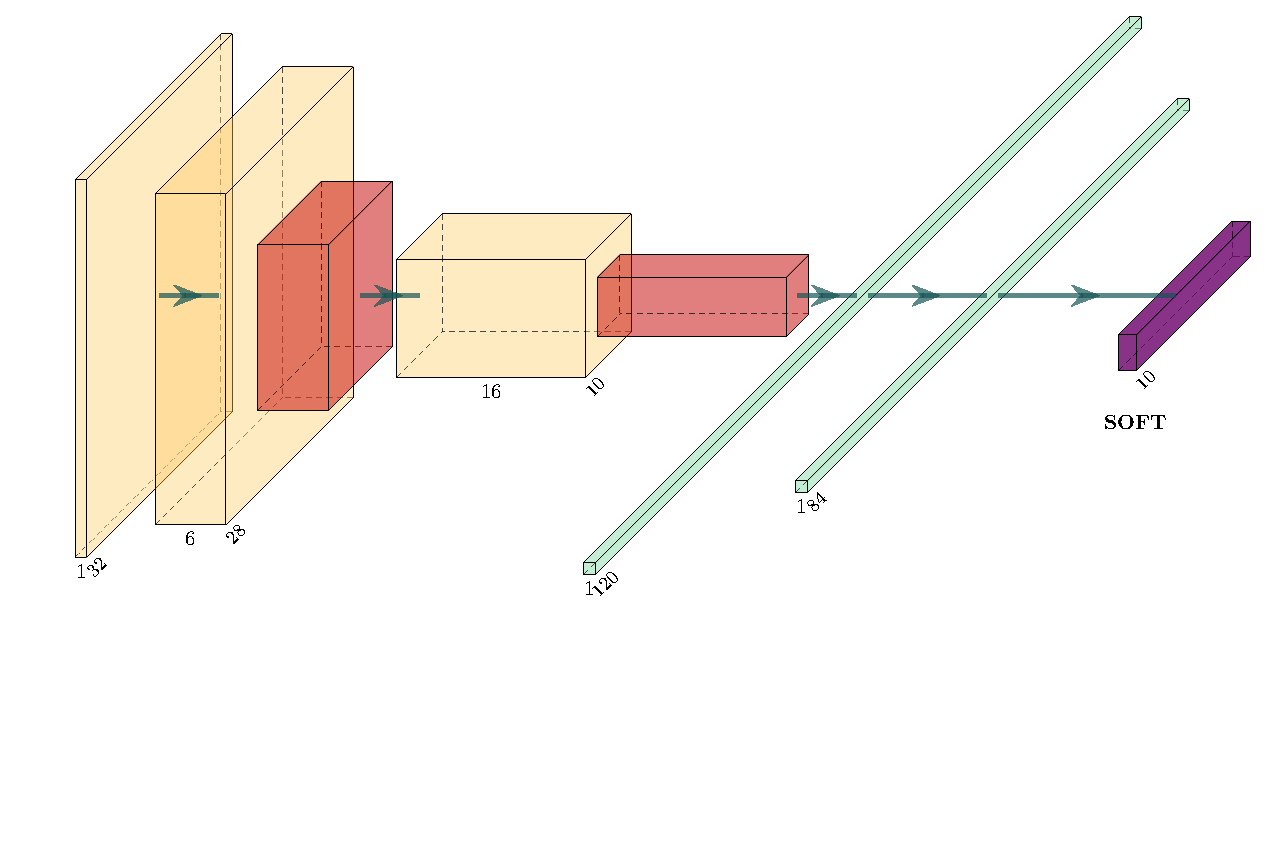
\includegraphics[width=0.8\textwidth]{src/lenet.pdf}
    \caption{Example of a simple CNN architecture (lenet.pdf) {ADD EXPLENATION}\cite{exCNN}}
\end{figure}


The first layers of the neural network consist of a hierarchy of convolution and pooling layers, each taking the output of the previous layer as input. The output of the final convolutional or pooling layer is then passed to a fully connected layer, which performs the final classification.

During training, the network first attempts to classify a batch of input elements. The predicted output is then compared to the true class labels, and a loss value is computed. This loss is subsequently backpropagated through the network, and the gradients for all learnable parameters are calculated. Finally, a step of gradient descent is performed, and the learnable parameters are updated accordingly.


\section{Networks used}

- two different architectures were used to classify the images: a LeNet-inspired CNN and an AlexNet-inspired CNN.
- both networks were trained on the same dataset, with the same hyperparameters, to ensure a fair comparison of their performance.


\subsection{LeNet-like network}

\begin{table}[h]
\centering
\caption{Architecture of the LeNet-inspired CNN model}
\label{tab:lenet_architecture}
\begin{tabular}{|l|c|c|}
\hline
\textbf{Layer} & \textbf{Output Shape} & \textbf{Details} \\
\hline
Input & \(1 \times H \times W\) & Input image \\
\hline
Conv2d (1 → 6) & \(6 \times (H-4) \times (W-4)\) & Kernel \(5 \times 5\), stride 1 \\
AvgPool2d & \(6 \times \frac{(H-4)}{2} \times \frac{(W-4)}{2}\) & Kernel \(2 \times 2\), stride 2 \\
\hline
Conv2d (6 → 16) & \(16 \times (H'-4) \times (W'-4)\) & \(H', W'\) from previous layer \\
AvgPool2d & \(16 \times \frac{(H'-4)}{2} \times \frac{(W'-4)}{2}\) & Kernel \(2 \times 2\), stride 2 \\
\hline
Conv2d (16 → 120) & \(120 \times 1 \times 1\) & Kernel \(5 \times 5\), stride 1 \\
\hline
Flatten & \(120\) & Vectorized output \\
Linear (120 → 84) & \(84\) & Fully connected + ReLU \\
Linear (84 → 2) & \(2\) & Output logits for classification \\
\hline
\end{tabular}
\end{table}

One of the architectures used was based on the classical LeNet-5 convolutional neural network, originally developed for digit recognition. It is a shallow network originally designed for small-scale image classification tasks.

The network consists of three convolutional layers. The first layer applies six \( 5 \times 5 \) kernels with stride 1, reducing the spatial resolution from \( H \times W \) to \( (H - 4) \times (W - 4) \). This is followed by a \( 2 \times 2 \) average pooling operation with stride 2, which halves the resolution in each spatial dimension. The second convolutional layer applies sixteen \( 5 \times 5 \) kernels, further reducing the spatial size, followed by another \( 2 \times 2 \) average pooling step. The final convolutional layer uses 120 filters of size \( 5 \times 5 \), resulting in an output of shape \( 120 \times 1 \times 1 \) for an appropriately sized input.

The output of the last convolution is flattened into a 120-dimensional vector and passed through two fully connected layers. The first has 84 hidden units followed by a ReLU activation function, and the second maps to the final two output classes.

This architecture is summarized in Table~\ref{tab:lenet_architecture}.


\subsection{AlexNet-Inspired CNN}


Another architecture utilized was a modified version of the AlexNet model, originally developed for the ImageNet Large Scale Visual Recognition Challenge (ILSVRC). The general hope being that the fact that it's significantly deeper and wider than LeNet would enable classify the images more effectively.

The network consists of five convolutional layers interspersed with batch normalization, ReLU activation functions, and max pooling operations. The first convolutional layer applies 64 filters of size \(11 \times 11\) with a stride of 4 and padding of 2, significantly reducing spatial dimensions early in the network. Subsequent layers progressively increase the channel depth and apply smaller kernels, maintaining resolution with padding. Batch normalization is used after each convolution to stabilize training.

After the convolutional blocks, the output is flattened and passed through three fully connected layers with 4096, 4096, and 2 units respectively. Dropout with a probability of 0.5 is applied between the fully connected layers to mitigate overfitting.

This architecture is summarized in Table~\ref{tab:alexnet_architecture}.

\begin{table}[h]
\centering
\caption{Architecture of the AlexNet-inspired CNN model}
\label{tab:alexnet_architecture}
\begin{tabular}{|l|c|c|}
\hline
\textbf{Layer} & \textbf{Output Shape} & \textbf{Details} \\
\hline
Input & \(1 \times H \times W\) & Variable-size input image \\
\hline
Conv2d (1 → 64) & Dependent on input & Kernel \(11 \times 11\), stride 4, padding 2 \\
BatchNorm2d & – & 64 feature maps \\
MaxPool2d & – & Kernel \(3 \times 3\), stride 2 \\
\hline
Conv2d (64 → 192) & – & Kernel \(5 \times 5\), padding 2 \\
BatchNorm2d & – & \\
MaxPool2d & – & Kernel \(3 \times 3\), stride 2 \\
\hline
Conv2d (192 → 384) & – & Kernel \(3 \times 3\), padding 1 \\
BatchNorm2d & – & \\
\hline
Conv2d (384 → 256) & – & Kernel \(3 \times 3\), padding 1 \\
BatchNorm2d & – & \\
\hline
Conv2d (256 → 256) & – & Kernel \(3 \times 3\), padding 1 \\
BatchNorm2d & – & \\
MaxPool2d & – & Kernel \(3 \times 3\), stride 2 \\
\hline
Flatten & – & Computed dynamically \\
Linear & \(4096\) & Fully connected + ReLU + Dropout \\
Linear & \(4096\) & Fully connected + ReLU + Dropout \\
Linear & \(2\) & Final output logits \\
\hline
\end{tabular}
\end{table}


\subsection{Model Training Procedure}

Both networks were trained using a training routine implemented in PyTorch. The training process operated on a combined dataset and dynamically inferred input dimensions from a sample image. Image preprocessing included optional downscaling using nearest-neighbor interpolation, followed by conversion to tensor format. The models were optimized using stochastic gradient descent (SGD) with a fixed learning rate of 0.0005 and a momentum of 0.9. Cross-entropy loss was used as the objective function. Training was conducted for 10 epochs with a batch size of 16. During each epoch, loss and classification accuracy were recorded.

The dataset was split into training, validation, and test sets in a 70/15/15 ratio. Networks were trained on the training set, and their performance was evaluated on the validation set. The best-performing model on the validation set was selected for final evaluation on the test set, which consisted of data the model had no access to previously. Training was conducted separately on the full dataset and on a subset limited to the top 50\% of most energetic lepton interactions. For simplicity, only data from plane2 was used. Input images were scaled down to 0.33 and 0.5 of their original size. Confusion matrices were computed for all trained models, and results were compared. F1 scores and ROC curves were calculated for the best-performing models.



\section{Results}
\subsection{performance on the validation set}

\subsubsection{LeNet}

\subsubsection{AlexNet}

\subsection{discussion}

- LeNet did not train at all on either of the datasets- all events were classified as just one class
- Alexnet perforemd significantly better, acheiving satisfactory results for both the full and the top50 datasets.
- Sclale factor did influenece the performance (the larger the image the better), but not very significantly.
- scale factor improved the networks ability to correctly classify events where no lepton shower was observerd.
- the most significant difference in performace between top50 and full can be observed when it comes to proper classification of no lepton interaction events.

\section{Transformer}

The transformer is a deep learning architecture introduced for processing sequential data, relying entirely on attention mechanisms and eliminating recurrence. It enables high parallelization and long-range dependency modeling, making it suitable for a wide range of tasks, including computer vision.

The core components of the transformer include multi-head self-attention layer and residual connections with layer normalization. The model is organized into repeated layers or blocks, each consisting of an attention sublayer (see Figure~\ref{fig:transformerEncoder}).

Inputs to the transformer are first passed through an embedding layer, and positional encodings are added to the embeddings to retain information about the order of tokens in the sequence. These embeddings are then passed through a number of encoder blocks, each consisting of multi-head self-attention and linear layers, with the output of one block serving as the input to the next. The final output is a sequence of continuous vectors, which can then be processed by a decoder or used directly for tasks such as classification or regression.

\subsection{Embeddings}

\begin{figure}[h]
    \centering
    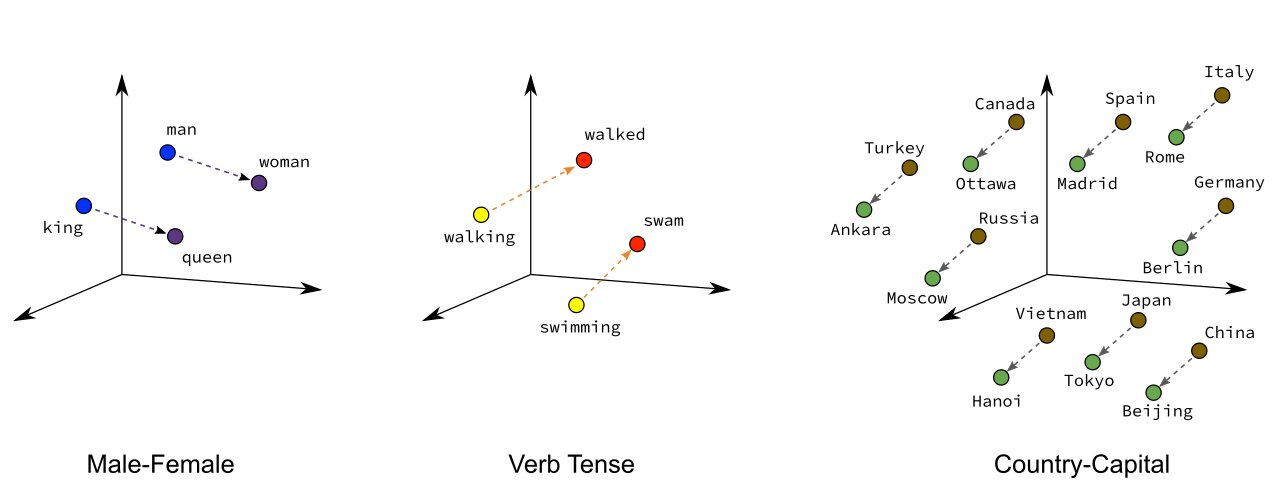
\includegraphics[width=0.9\textwidth]{src/word_embeddings_semantics.png}
    \caption{A simplified example of word embeddings projected into three dimensions. Words that share functional or structural roles—such as verb tense or country-capital pairs—tend to form consistent spatial patterns.}
    \label{fig:embedding_example}
\end{figure}

Transformer-based architectures operate on continuous vector representations. For this reason, each input passed into the network—also known as a token—must be mapped to a fixed-dimensional dense vector, known as an embedding. An example of word embeddings in a low-dimensional space is shown in Figure~\ref{fig:embedding_example}.

Formally, for an input consisting of \( V \) tokens and an embedding dimension \( d \), the embedding layer is represented by a matrix \( \mathbf{E} \in \mathbb{R}^{V \times d} \).

Given a sequence of input tokens \( \{t_1, t_2, \ldots, t_n\} \), the corresponding embedding vectors \( \{\mathbf{x}_1, \mathbf{x}_2, \ldots, \mathbf{x}_n\} \) are obtained by indexing into the embedding matrix:
\[
\mathbf{x}_i = \mathbf{E}[t_i] \in \mathbb{R}^d
\]

The embedding matrix consists of trainable parameters and is optimized jointly with the rest of the model. The goal of this mapping is to project discrete inputs into a continuous space where meaningful relationships can be learned during training.

\subsection{Transformer Encoder}

\begin{figure}[h]
    \centering
    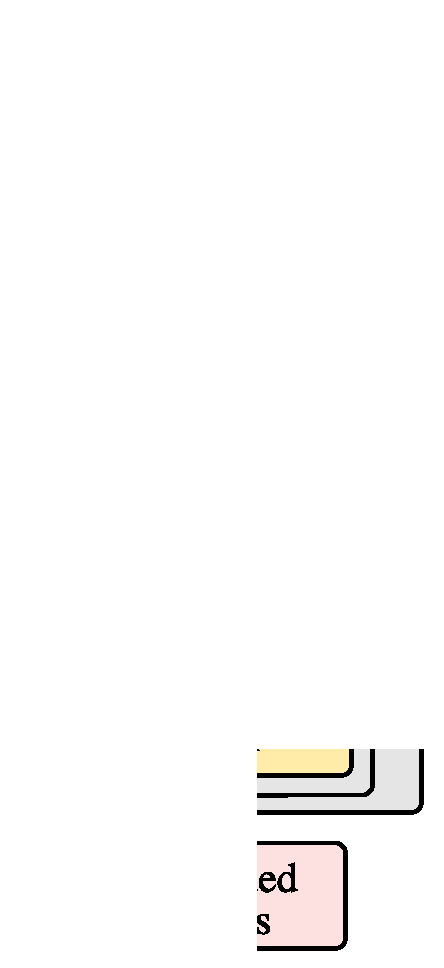
\includegraphics[width=0.2\textwidth]{src/transformerEncoder.pdf}
    \caption{Visual representation of a transformer block.}
    \label{fig:transformerEncoder}
\end{figure}

This structure is referred to as an encoder block and is visualized in Figure~\ref{fig:transformerEncoder}. In the transformer architecture, the self-attention mechanism—specifically multi-head attention—is a central component that enables the model to attend to different parts of the input sequence simultaneously.

\subsection{Single attention head}

\begin{figure}[h]
    \centering
    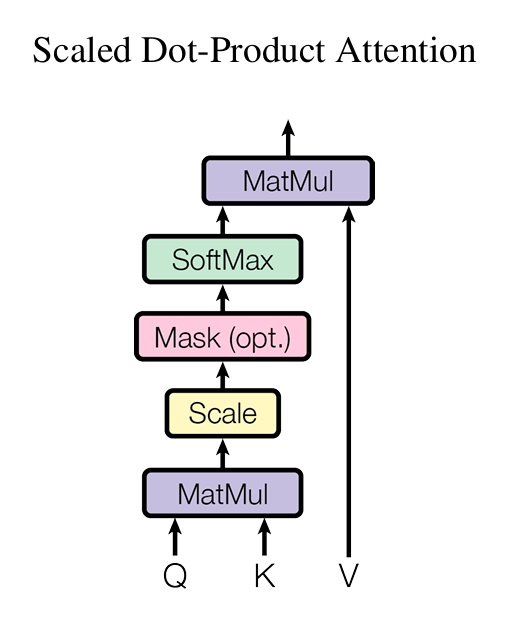
\includegraphics[width=0.5\textwidth]{src/scaledDotProd.png}
    \caption{Graphic representation of a single attention head. The input query, key, and value matrices are passed through a scaled dot-product attention mechanism, which computes attention scores and produces the output.}
    \label{fig:singleAttentionHead}
\end{figure}

The mechanism of a single attention head is illustrated in Figure~\ref{fig:singleAttentionHead}.


Each attention head receives three inputs: the query vector \( Q \in \mathbb{R}^{n \times d_k} \), the key matrix \( K \in \mathbb{R}^{n \times d_k} \), and the value matrix \( V \in \mathbb{R}^{n \times d_v} \), where \( n \) is the sequence length, and \( d_k \), \( d_v \) are the dimensionalities of the key and value vectors, respectively. The attention operation begins by computing a score vector through the dot product of the query and the transpose of the key matrix:
\[
\text{scores} = QK^\top
\]
This score vector is then scaled and passed through a softmax function to yield attention weights:
\[
\text{weights} = \text{softmax}\left(\frac{\text{scores}}{\sqrt{d_k}}\right)
\]
These weights are subsequently used to compute a weighted sum of the value vectors, producing the output of the attention head:
\[
\text{Attention}(Q, K, V) = \text{weights} \cdot V
\]

\subsection{Multi-head attention}

\begin{figure}[h]
    \centering
    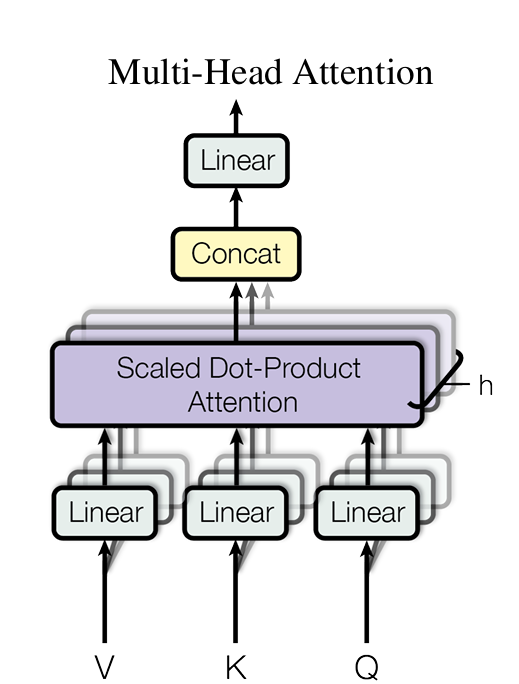
\includegraphics[width=0.5\textwidth]{src/multiHead.png}
    \caption{Graphic representation of a multi-head attention mechanism. The input query, key, and value matrices are passed through multiple independent attention heads, each computing its own attention output. The outputs of all heads are concatenated and projected back to the original dimensionality.}
    \label{fig:multiHeadAttention}
\end{figure}

A visual overview of the multi-head attention mechanism is provided in Figure~\ref{fig:multiHeadAttention}.


The multi-head attention mechanism extends the single-head idea by introducing multiple independent attention heads. Before attention is computed, the original input matrices \( Q \), \( K \), and \( V \) are each passed through separate trainable linear projections.

Instead of applying a single attention function with \( d_{\text{model}} \)-dimensional queries, keys, and values, the multi-head attention mechanism projects the inputs into multiple lower-dimensional subspaces and performs attention in parallel across these subspaces.

Specifically, for each attention head \( i \in \{1, \dots, h\} \), the queries \( Q \), keys \( K \), and values \( V \) are linearly projected using trainable weight matrices:
\[
QW_i^Q \in \mathbb{R}^{n \times d_k}, \quad KW_i^K \in \mathbb{R}^{n \times d_k}, \quad VW_i^V \in \mathbb{R}^{n \times d_v}
\]
Each attention head computes scaled dot-product attention independently:
\[
\text{head}_i = \text{Attention}(QW_i^Q, KW_i^K, VW_i^V)
\]

The outputs of all attention heads are then concatenated along the feature dimension:
\[
\text{MultiHead}(Q, K, V) = \text{Concat}(\text{head}_1, \ldots, \text{head}_h)W^O
\]
where \( W^O \in \mathbb{R}^{hd_v \times d_{\text{model}}} \).

The matrices \( W^Q_i \), \( W^K_i \), \( W^V_i \), and \( W^O \) consist of trainable parameters optimized during training.s

\subsection{Residual connections and layer normalization}

\begin{figure}[h]
    \centering
    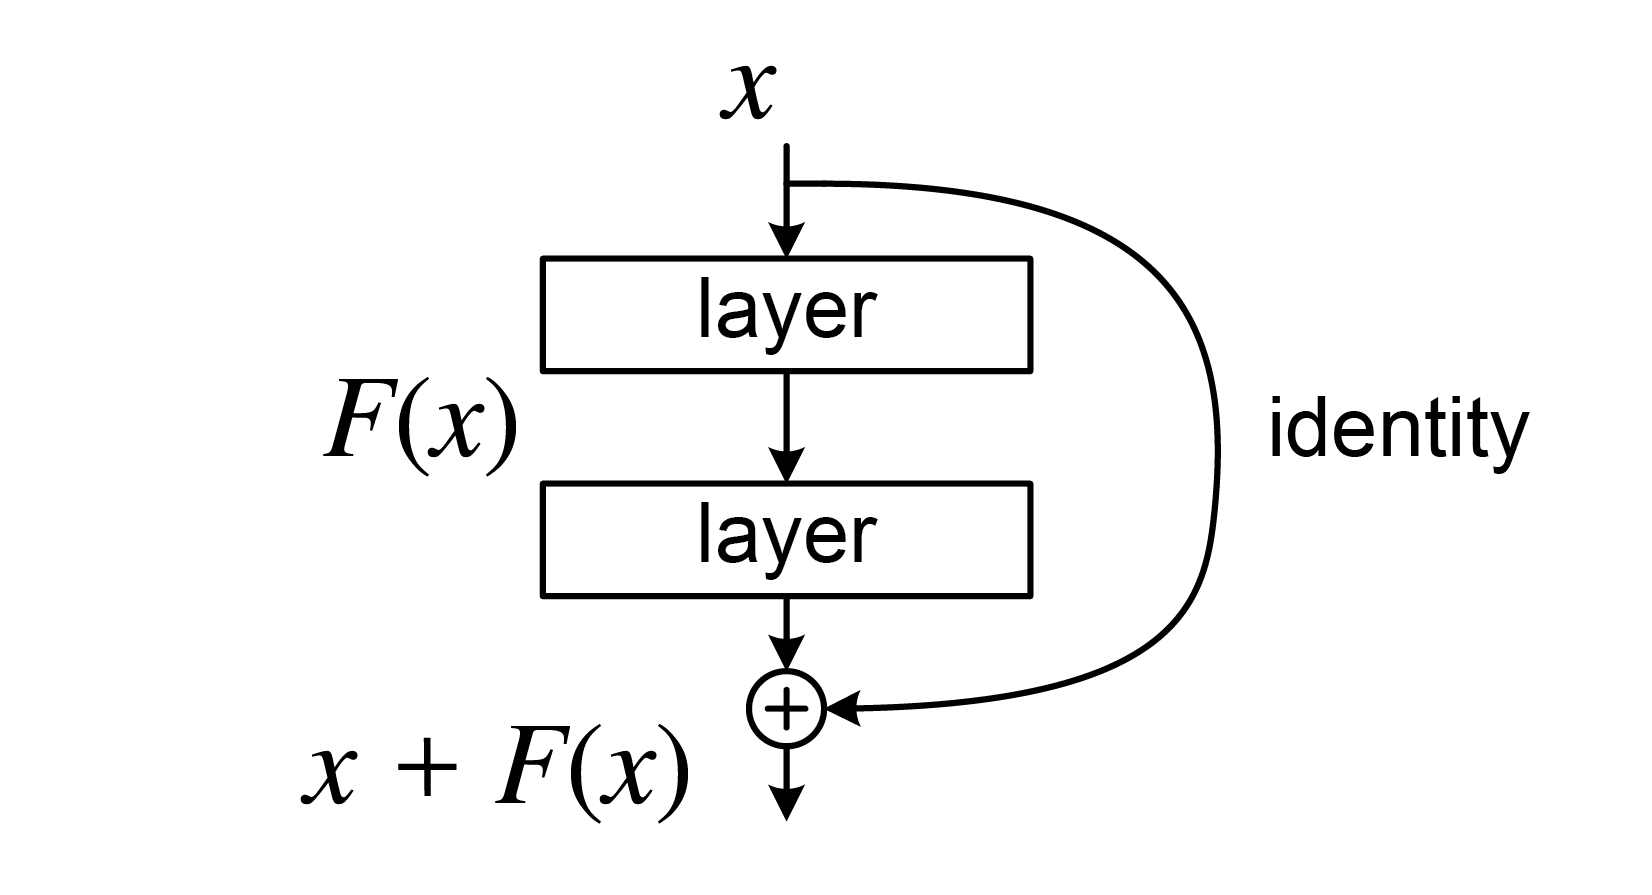
\includegraphics[width=0.6\textwidth]{src/ResBlock.png}
    \caption{Graphic representation of a residual connection.}
    \label{fig:resCon}
\end{figure}

The residual connection and normalization process are shown in Figure~\ref{fig:resCon}.

To facilitate stable training and improve gradient flow, the transformer applies residual connections around each sublayer, followed by layer normalization.

Given an input \( \mathbf{x} \) and a sublayer function \( \text{Sublayer}(\cdot) \), the output is computed as:
\[
\text{LayerNorm}(\mathbf{x} + \text{Sublayer}(\mathbf{x}))
\]

The residual connection adds the input of the sublayer to its output, and layer normalization standardizes the summed output across the feature dimension. This structure helps preserve information and stabilizes the optimization process.


\subsection{Positional encoding}

\begin{figure}[H]
    \centering
    \begin{minipage}{0.49\textwidth}
        \centering
        \begin{align*}
        PE(pos, 2i) &= \sin\left(\frac{pos}{10000^{\frac{2i}{d_{\text{model}}}}}\right) \\
        PE(pos, 2i + 1) &= \cos\left(\frac{pos}{10000^{\frac{2i}{d_{\text{model}}}}}\right)
        \end{align*}
    \end{minipage}
    \begin{minipage}{0.49\textwidth}
        \centering
        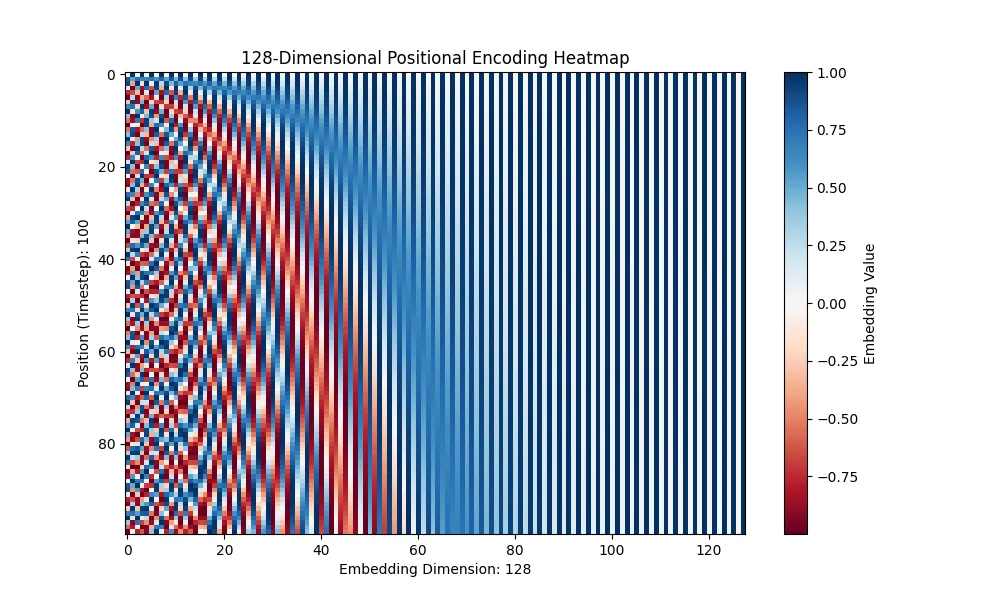
\includegraphics[width=0.9\textwidth]{src/embedings.png}
    \end{minipage}
    \caption{Example of how positional encoding can be handled. The heatmap on the right visually represents a positional encoding for 128-dimensional vectors. Each row corresponds to a position in the input sequence, and each column represents a dimension within the embedding vector. The color gradient signifies the value of the positional encoding at that specific position and dimension. The equations on the left define the sinusoidal functions used to compute the positional encoding for each position \( pos \) and dimension \( i \) in the embedding vector.}
\end{figure}

The sinusoidal positional encoding and its heatmap representation are shown in the diagram in Figure~\ref{fig:positionalEncoding}.


Importantly, the architecture described above does not inherently retain positional information of the input sequence. To address this, the transformer architecture incorporates \textit{positional encoding}, which injects information about the position of each token in the sequence into the input embeddings. The encoded position of each token is added to its corresponding embedding before being passed through the transformer layers:
\[
\mathbf{z}_0 = \mathbf{x} + \mathbf{P}
\]
where \( \mathbf{x} \) denotes the input embedding and \( \mathbf{P} \) is the positional encoding.

\section{Image Transformer}

\subsection{Image Transformer Architecture}

\begin{figure}[h]
    \centering
    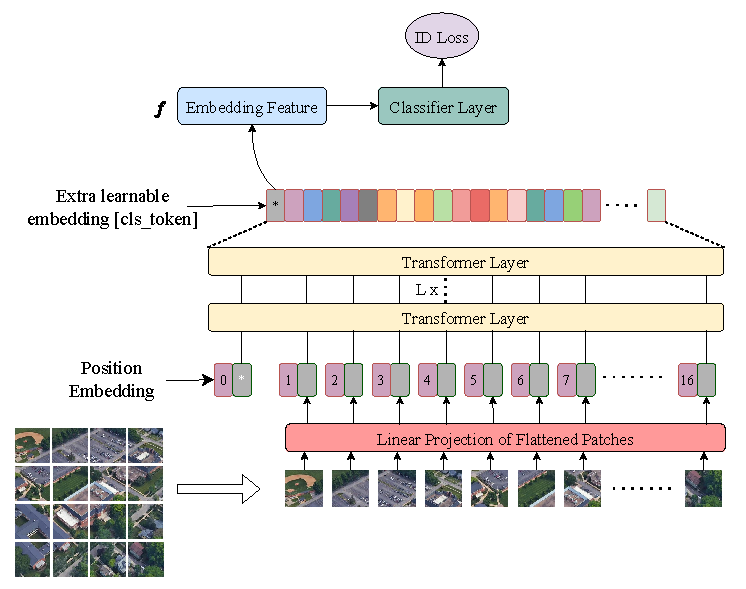
\includegraphics[width=0.55\textwidth]{src/visNet.pdf}
    \caption{Visual transformer architecture visualized}
    \label{fig:visNetArch}
\end{figure}

The transformer architecture adapted for images is illustrated in Figure~\ref{fig:visNetArch}.


The image transformer extends the standard transformer architecture to process visual inputs. Rather than operating on word tokens, the input image is divided into a sequence of fixed-size non-overlapping patches. A typical configuration involves splitting the image into 16 patches of \(16 \times 16\) pixels each. These patches are then flattened into vectors and linearly projected to a fixed embedding dimension, producing a sequence of patch embeddings.

Each patch embedding is augmented with a corresponding positional embedding to encode spatial location. This sequence is then processed by a stack of transformer encoder layers, each comprising multi-head self-attention and feed-forward sublayers with residual connections and layer normalization. The transformer outputs a set of encoded vectors, which are subsequently used for downstream tasks such as classification or detection.

\subsection{Classification Token}

To enable image-level classification, a special token known as the classification token, or [CLS] token, is prepended to the sequence of patch embeddings. This token does not represent any specific region of the image and is initialized as a trainable vector. Throughout the transformer layers, it interacts with other tokens via the self-attention mechanism and gradually aggregates global information about the entire image.

After processing through all transformer layers, the final output corresponding to the [CLS] token serves as a global representation of the image. This output is passed to a multi-layer perceptron (MLP) head to produce class logits. The [CLS] token is trained jointly with the model to optimize performance on the target classification task.

\subsection{Positional Encoding for Image Fragments}

\begin{figure}[h]
    \centering
    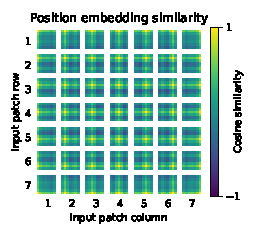
\includegraphics[width=0.45\textwidth]{src/imNetEncodings.pdf}
    \caption{Cosine similarity of positional encoding for image patches from the original Vision Transformer paper. Embeddings for patches close to each other are similar.}
    \label{fig:imNetEncodings}
\end{figure}

Figure~\ref{fig:imNetEncodings} shows how positional encodings correlate spatially in image transformers.


To retain spatial context after converting image patches into a sequence, positional embeddings are added to each patch embedding. These embeddings are learnable parameters and are optimized during training alongside the rest of the model. Their purpose is to encode the location of each patch within the original image, enabling the model to distinguish between otherwise identical patches in different positions.

Empirical analysis has shown that these embeddings evolve such that neighboring patches in the image space tend to receive similar positional encodings. This spatial correlation helps the transformer capture local structure while also enabling long-range dependencies to be modeled across distant regions of the image.


\section{Transformer architecture used}

The specific transforemer image transformer that ended up being used divided images into patches of 16x16 pixels each. Each patch is mapped to a 32-dimensional embedding vector. Positional encoding is applied using sine and cosine functions across the embedding dimensions. The model includes a single multi-head self-attention layer with two heads to capture relationships between patches. A final three-layer multilayer perceptron consisted of layer sizes of 32, 16, and 2 neurons respectively.

\subsection{Training procedure}

The transformer was trained for up to 10 epochs using a dataset split into training and validation batches. The validation set consisted of 1000 batches taken from the dataset, while the rest was used for training. An Adam optimizer with an exponentially decaying learning rate starting at 0.001 was used, with the learning rate decreasing by 5\% every 10 full passes through the training data. The model optimized a binary cross-entropy loss and tracked accuracy as a metric. Training incorporated early stopping, halting if the validation accuracy did not improve for 10 consecutive epochs.

\section{Transformer theirraining and Evaluation Results}


\subsection{Training Summary}

The neural network was trained for 10 epochs using an exponentially decaying learning rate schedule. The final training loss reached \textbf{0.5839}, with a training accuracy of \textbf{69.04\%}. Validation performance at the end of training showed a loss of \textbf{0.6139} and an accuracy of \textbf{66.00\%}, which was also the best recorded validation accuracy.

Testing on the held-out dataset yielded a final loss of \textbf{0.6218} and an accuracy of \textbf{66.03\%}, indicating consistent generalization performance.

\subsection{Learning Dynamics}

During training, the loss decreased by \textbf{12.0\%}, and accuracy improved by \textbf{9.75 percentage points}. The training-validation accuracy gap was \textbf{3.04 percentage points}, suggesting low overfitting. Loss fluctuations over the final five epochs were minimal (standard deviation: \textbf{0.0039}), indicating moderate convergence.

\subsection{Classification Metrics}

Evaluation of class-wise performance yielded the following:

\begin{itemize}
    \item \textbf{Class "CC e"}
    \begin{itemize}
        \item Precision: 0.6773
        \item Recall: 0.6442
        \item F1-Score: 0.6603
    \end{itemize}
    \item \textbf{Class "other"}
    \begin{itemize}
        \item Precision: 0.6441
        \item Recall: 0.6773
        \item F1-Score: 0.6603
    \end{itemize}
\end{itemize}

The overall model achieved an \textbf{AUC-ROC score of 0.7207}, confirming its capacity to discriminate between the two classes effectively.

\subsection{Confusion Matrix}

Figure~\ref{fig:conf_matrix} presents the normalized confusion matrix for the test set. The model correctly classified \textbf{64\%} of "CC e" instances and \textbf{68\%} of "other" instances. Misclassification rates were relatively balanced between the two classes.

\begin{figure}[H]
    \centering
    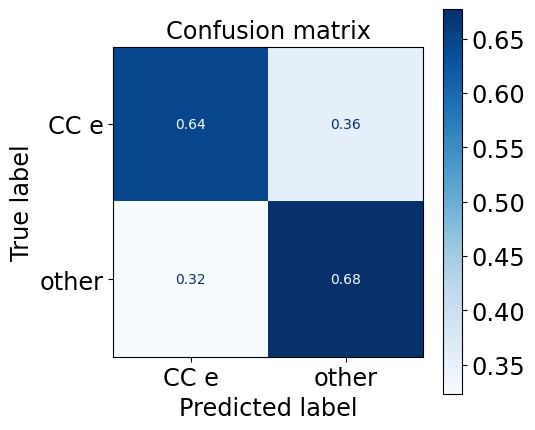
\includegraphics[width=0.45\textwidth]{src/tranformerMatrixFinal.png}
    \caption{Normalized confusion matrix showing prediction distribution across classes.}
    \label{fig:conf_matrix}
\end{figure}


\section{Conclusion}

\newpage

\section{Bibliography}
\bibliographystyle{plain}
\bibliography{references}

\end{document}